\documentclass[10pt,a4paper]{article}

\usepackage[T1]{fontenc}
\usepackage{lmodern}
\usepackage[margin=2cm]{geometry}
\usepackage{microtype}
\usepackage{amsmath}
\usepackage{booktabs,tabularx,longtable,array}
\usepackage[table]{xcolor}
\usepackage{enumitem}
\usepackage{float}
\usepackage[font=small,skip=4pt]{caption}
\usepackage{parskip}
\usepackage{titlesec}
\usepackage{pdflscape}
\usepackage{tikz}
\usetikzlibrary{positioning,arrows.meta,shapes.geometric,shapes.misc,fit,backgrounds,calc}
\usepackage[colorlinks=true,linkcolor=blue!50!black,urlcolor=blue!50!black]{hyperref}

\makeatletter
\g@addto@macro{\UrlBreaks}{\do\/\do-\do\_\do\?\do\=\do\&\do\.\do\a\do\b\do\c\do\d\do\e\do\f\do\g\do\h\do\i\do\j\do\k\do\l\do\m\do\n\do\o\do\p\do\q\do\r\do\s\do\t\do\u\do\v\do\w\do\x\do\y\do\z}
\makeatother

\definecolor{kfcblue}{HTML}{185FA5}
\definecolor{kfcteal}{HTML}{0F6E56}
\definecolor{kfcpurple}{HTML}{534AB7}
\definecolor{kfcgray}{HTML}{5F5E5A}
\definecolor{lightblue}{HTML}{E6F1FB}
\definecolor{lightteal}{HTML}{E1F5EE}
\definecolor{lightpurple}{HTML}{EEEDFE}
\definecolor{lightgray}{HTML}{F1EFE8}
\definecolor{lightamber}{HTML}{FAEEDA}

\titleformat{\section}{\large\bfseries\color{kfcblue}}{\thesection}{0.6em}{}
\titleformat{\subsection}{\normalsize\bfseries}{\thesubsection}{0.6em}{}
\titlespacing*{\section}{0pt}{10pt}{4pt}
\titlespacing*{\subsection}{0pt}{6pt}{2pt}
\setlist{itemsep=1pt,topsep=2pt,parsep=0pt}
\renewcommand{\arraystretch}{1.15}
\newcolumntype{L}[1]{>{\raggedright\arraybackslash}p{#1}}
\newcolumntype{Y}{>{\raggedright\arraybackslash}X}
\pagestyle{plain}

\newcommand{\ep}[1]{\texttt{\small #1}}
\newcommand{\eu}[1]{{\small\nolinkurl{#1}}}
\newcommand{\todo}[1]{\textbf{[TODO: #1]}}

\begin{document}

\begin{titlepage}
\centering
\vspace*{\fill}
{\Huge\bfseries\color{kfcblue} GameTrend Radar\par}
\vspace{0.4cm}
{\Large Real-time trend analytics for Roblox and Steam games\par}
\vspace{0.3cm}
{\large Project Milestone 2: data acquisition and pre-processing\par}
\vspace{2.5cm}
{\Large\bfseries Team KFC\par}
\vspace{0.5cm}
{\large
Bart\l{}omiej Borycki\\[3pt]
Micha\l{} Iwaniuk\\[3pt]
Jan Cwalina\\[3pt]
Mi\l{}osz Choda\'n\par}
\vspace*{\fill}
\end{titlepage}

\tableofcontents
\newpage

%======================================================================
\section{Project deliverables (user's perspective)}\label{sec:deliverables}
Roblox is a trend-driven game platform with a young audience (mostly 10--15 years old). New mechanics spread within days, and many of them are copied from Steam hits. Our users are independent Roblox developers, small studios and game-market analysts. They want to know what is rising now, where a trend came from, and how crowded a niche is.

\begin{itemize}
  \item A web dashboard with four views: \emph{Trending now} (the entry point of the core use case), \emph{Game details}, \emph{Steam$\rightarrow$Roblox opportunities} and \emph{Model and data health}. Section~\ref{sec:presentation} describes them.
  \item A data platform in a lambda architecture, run locally with Docker Compose.
  \item Two linear regressions in Spark MLlib: an expected-players model for Roblox, whose ratio of actual to expected players is the trend score, and a +3\,h player projection evaluated against two simple baselines.
\end{itemize}
We collect only aggregated, public, game-level data and store nothing about individual players.

%======================================================================
\section{Business process -- core use case}\label{sec:process}
The core use case is ``monitor trending Roblox games and find where a trend came from'' (Figure~\ref{fig:bpmn}). The developer opens \emph{Trending now}, filters it by genre and opens a Roblox game with a high trend score or growth. Its details show the player history, the trend score and the +3\,h projection. If the game has a possible Steam counterpart, the developer reviews that Steam game's growth and the other Roblox games matched to it, which shows how crowded the niche is. Otherwise the trend has no detected Steam origin, and the assessment relies on the Roblox metrics alone. Matching indicates possible counterparts, not verified copying. The \emph{Steam$\rightarrow$Roblox opportunities} view remains as a supplementary entry point for browsing from the Steam side. Figure~\ref{fig:interaction-overview} shows the same flow across the dashboard and the data platform.

\begin{landscape}
\begin{figure}[p]
\centering
\resizebox{\linewidth}{!}{% BPMN: monitor a trending Roblox game and trace its possible Steam origin.
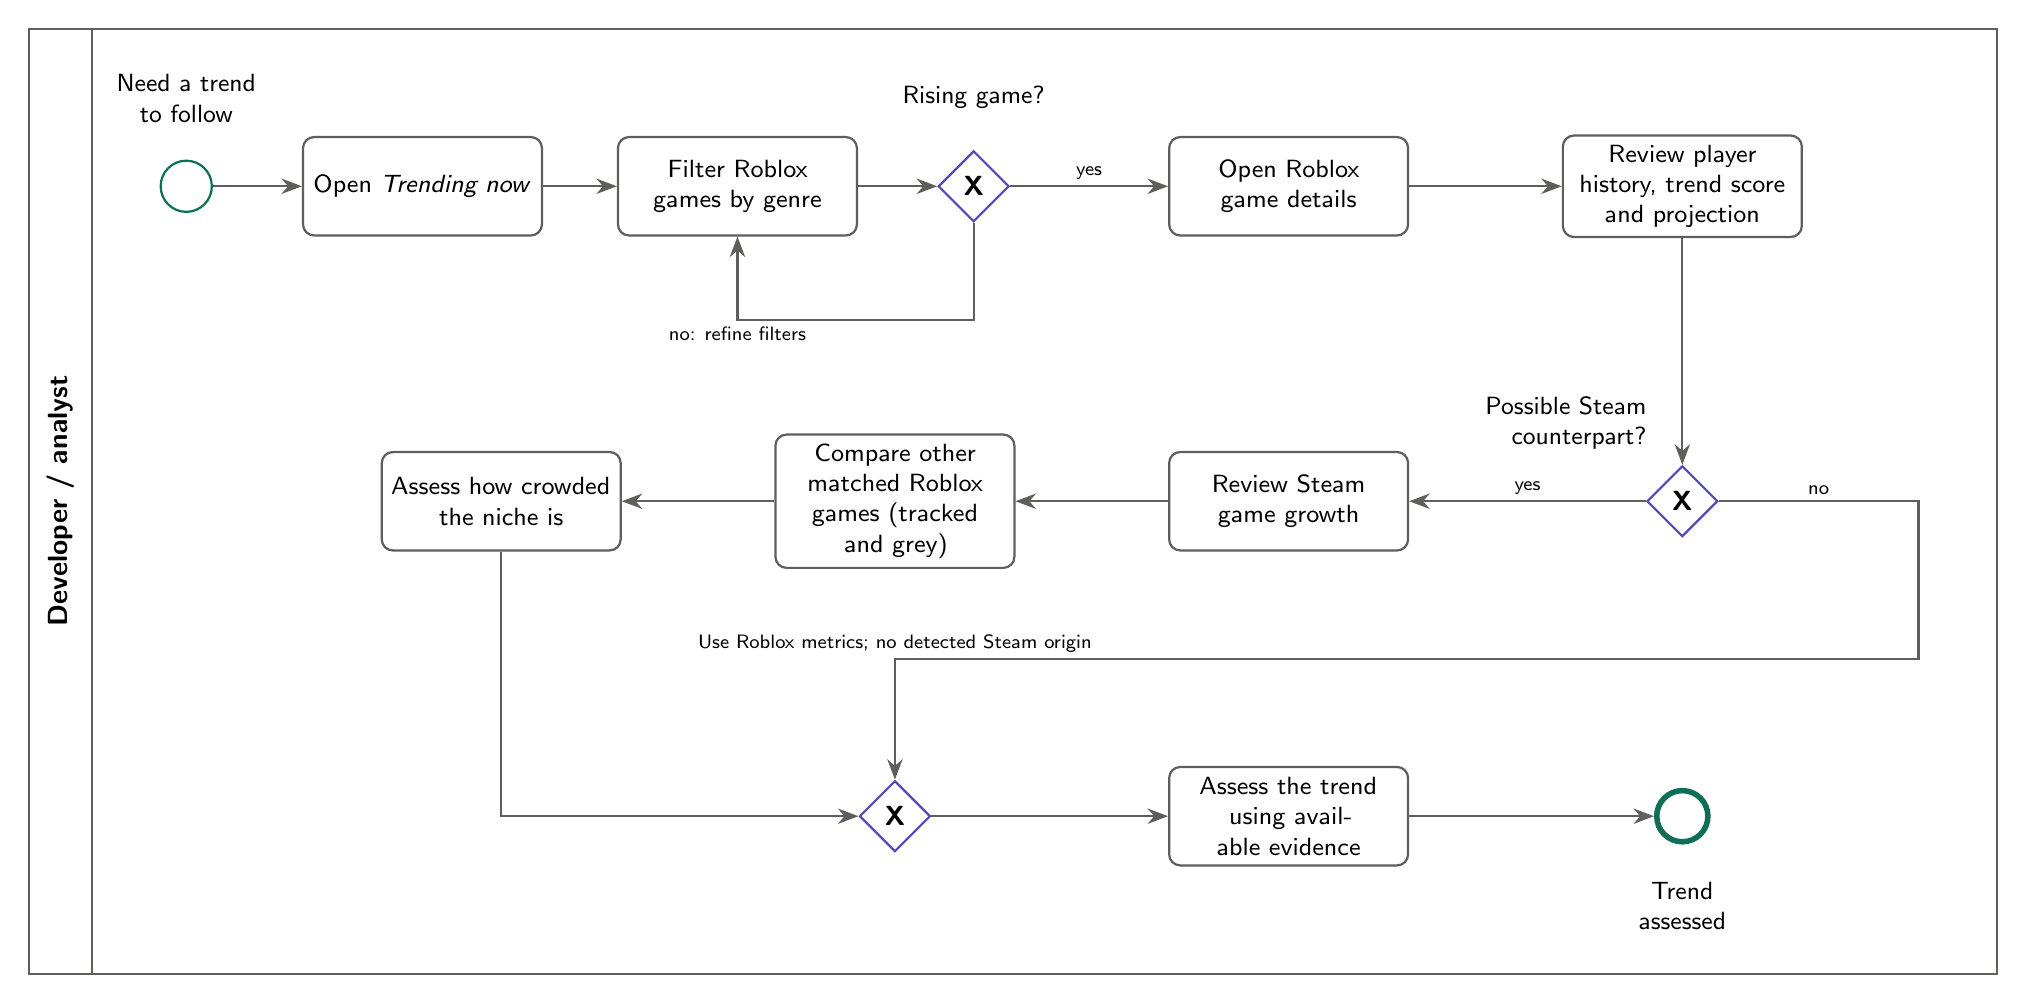
\begin{tikzpicture}[
  font=\sffamily\small,
  task/.style={rectangle, rounded corners=4pt, draw=kfcgray, fill=white, thick, minimum height=1.25cm, align=center, text width=2.8cm},
  start/.style={circle, draw=kfcteal, thick, minimum size=0.65cm, fill=white},
  endev/.style={circle, draw=kfcteal, line width=2pt, minimum size=0.65cm, fill=white},
  gw/.style={diamond, draw=kfcpurple, thick, fill=white, minimum size=0.9cm, inner sep=0pt, font=\sffamily\bfseries},
  flow/.style={-{Stealth[length=2.6mm]}, thick, draw=kfcgray},
  lbl/.style={font=\sffamily\scriptsize, fill=white, inner sep=2pt}
]
\draw[thick, kfcgray] (0,0) rectangle (25,-12);
\draw[thick, kfcgray] (0.8,0) -- (0.8,-12);
\node[rotate=90, font=\sffamily\bfseries] at (0.4,-6) {Developer / analyst};

\node[start] (start) at (2,-2) {};
\node[above=0.35cm of start, align=center] {Need a trend\\to follow};
\node[task] (browse) at (5,-2) {Open \emph{Trending now}};
\node[task] (filter) at (9,-2) {Filter Roblox games by genre};
\node[gw] (rising) at (12,-2) {X};
\node[above=0.4cm of rising] {Rising game?};
\node[task] (details) at (16,-2) {Open Roblox game details};
\node[task] (metrics) at (21,-2) {Review player history, trend score and projection};

\node[gw] (linked) at (21,-6) {X};
\node[above left=0.3cm and 0.1cm of linked, align=right] {Possible Steam\\counterpart?};
\node[task] (steam) at (16,-6) {Review Steam game growth};
\node[task] (others) at (11,-6) {Compare other matched Roblox games (tracked and grey)};
\node[task] (niche) at (6,-6) {Assess how crowded the niche is};
\node[gw] (merge) at (11,-10) {X};
\node[task] (assess) at (16,-10) {Assess the trend using available evidence};
\node[endev] (end) at (21,-10) {};
\node[below=0.35cm of end, align=center] {Trend\\assessed};

\draw[flow] (start) -- (browse);
\draw[flow] (browse) -- (filter);
\draw[flow] (filter) -- (rising);
\draw[flow] (rising) -- node[lbl, above]{yes} (details);
\draw[flow] (rising.south) -- (12,-3.7) -| node[lbl, pos=0.5, below]{no: refine filters} (filter.south);
\draw[flow] (details) -- (metrics);
\draw[flow] (metrics) -- (linked);
\draw[flow] (linked) -- node[lbl, above]{yes} (steam);
\draw[flow] (steam) -- (others);
\draw[flow] (others) -- (niche);
\draw[flow] (niche.south) |- (merge.west);
\draw[flow] (linked.east) -- node[lbl, above]{no} (24,-6) -- (24,-8) -| node[lbl, pos=0.5, above]{Use Roblox metrics; no detected Steam origin} (merge.north);
\draw[flow] (merge) -- (assess);
\draw[flow] (assess) -- (end);
\end{tikzpicture}
}
\caption{BPMN business process for monitoring a trending Roblox game and tracing its Steam origin (one participant; diamonds are exclusive gateways).}
\label{fig:bpmn}
\end{figure}
\end{landscape}

\begin{landscape}
\begin{figure}[p]
\centering
\resizebox{\linewidth}{!}{% Interaction overview of the core use case across user, dashboard and data platform; conceptual notation, not formal BPMN.
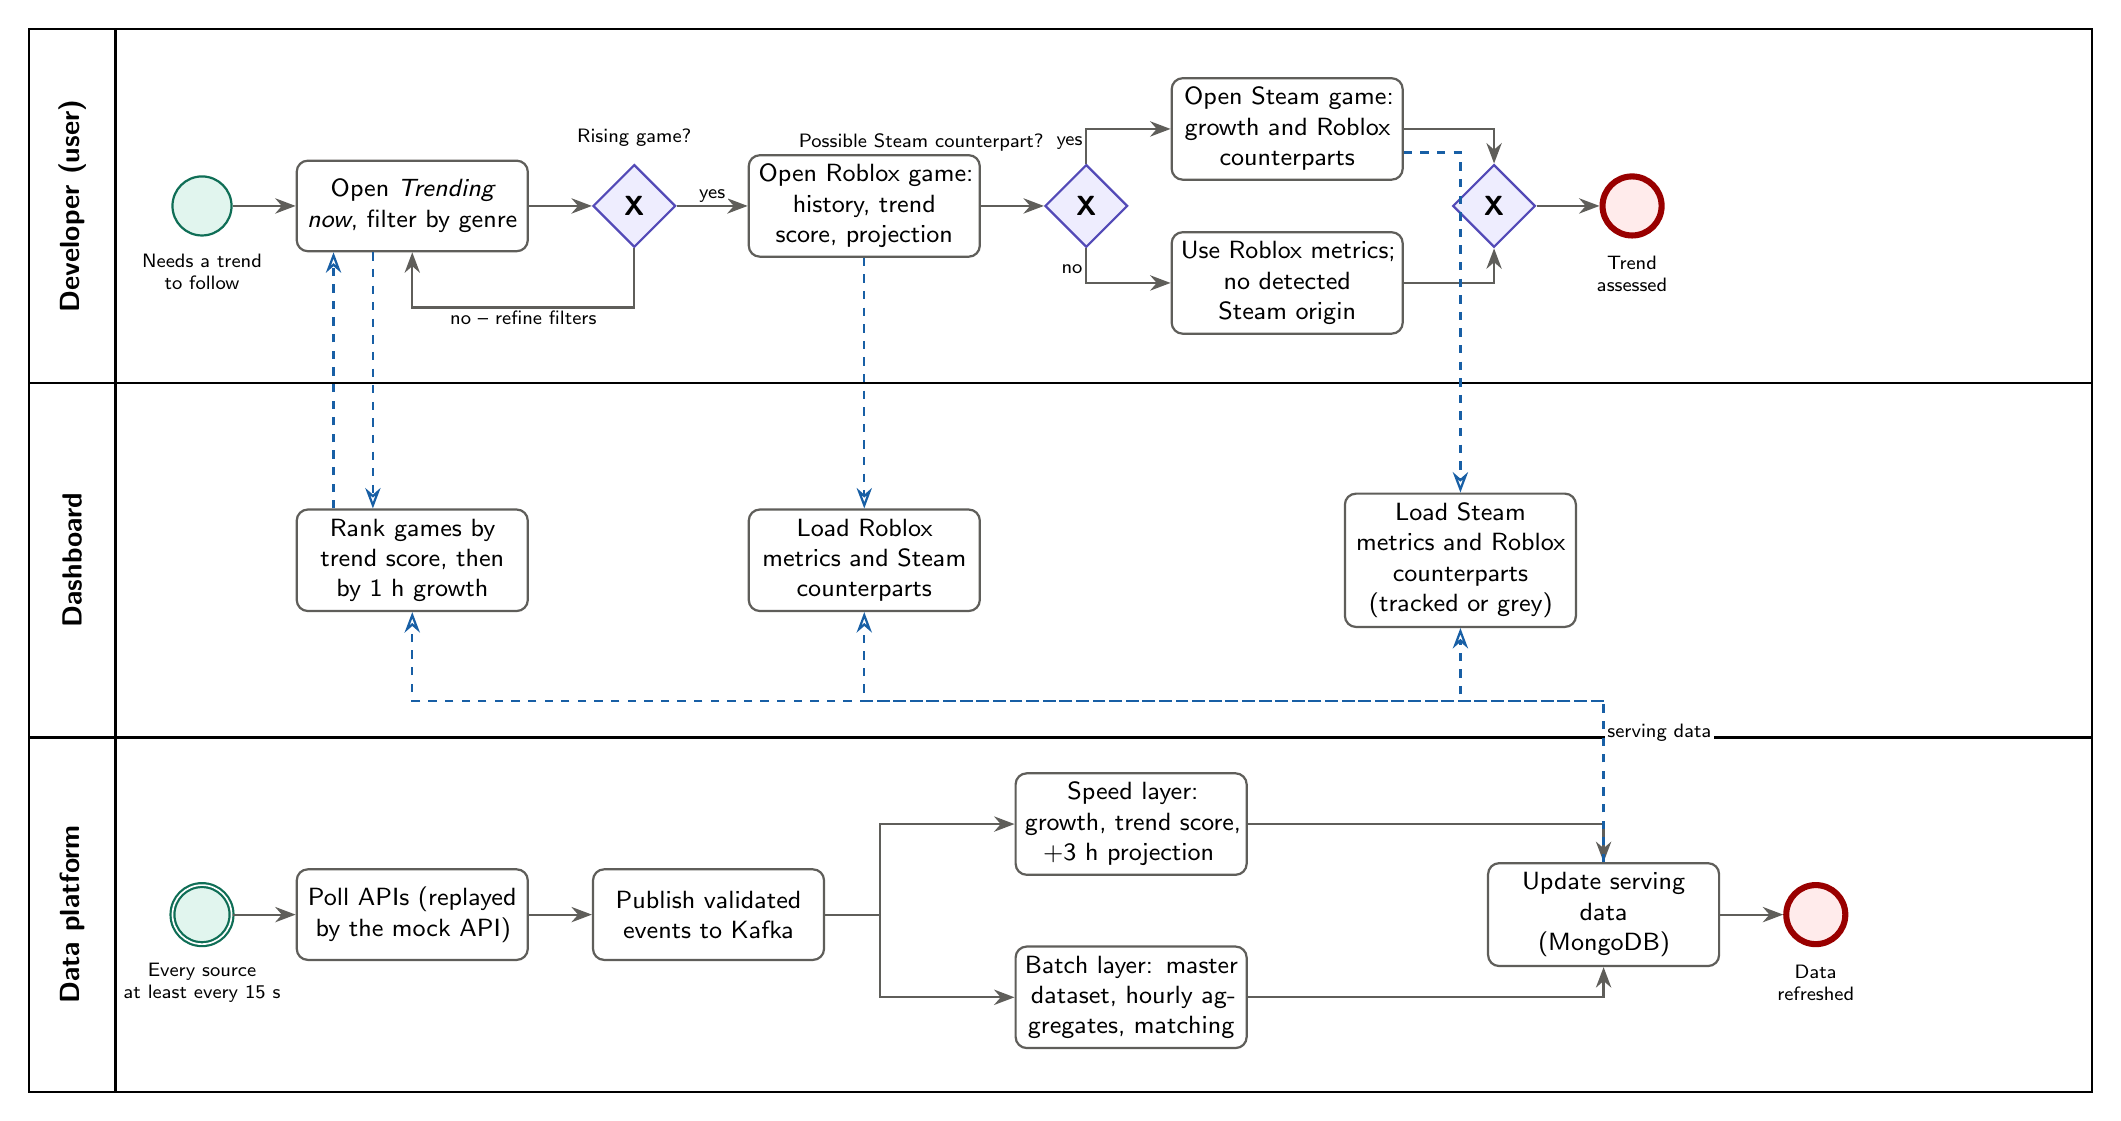
\begin{tikzpicture}[
  font=\sffamily\small,
  task/.style={rectangle, rounded corners=4pt, draw=kfcgray, fill=white, thick, minimum width=2.9cm, minimum height=1.15cm, align=center, text width=2.7cm},
  start/.style={circle, draw=kfcteal, thick, minimum size=0.75cm, fill=lightteal},
  timer/.style={circle, draw=kfcteal, double, thick, minimum size=0.75cm, fill=lightteal},
  endev/.style={circle, draw=red!60!black, line width=2.2pt, minimum size=0.75cm, fill=red!8},
  gw/.style={diamond, draw=kfcpurple, thick, fill=lightpurple, minimum size=1.05cm, inner sep=0pt, font=\sffamily\bfseries},
  flow/.style={-{Stealth[length=2.6mm]}, thick, draw=kfcgray},
  msg/.style={-{Stealth[length=2.6mm,open]}, dashed, thick, draw=kfcblue},
  lbl/.style={font=\sffamily\scriptsize, fill=white, inner sep=1pt}
]
% lanes
\def\W{26.2}
\draw[thick] (0,0) rectangle (\W,-13.5);
\draw[thick] (0,-4.5) -- (\W,-4.5);
\draw[thick] (0,-9) -- (\W,-9);
\draw[thick] (1.1,0) -- (1.1,-13.5);
\node[rotate=90, font=\sffamily\bfseries] at (0.55,-2.25) {Developer (user)};
\node[rotate=90, font=\sffamily\bfseries] at (0.55,-6.75) {Dashboard};
\node[rotate=90, font=\sffamily\bfseries] at (0.55,-11.25) {Data platform};

% ---- user lane
\node[start] (s) at (2.2,-2.25) {};
\node[below=1mm of s, font=\sffamily\scriptsize, align=center] {Needs a trend\\to follow};
\node[task, right=0.8cm of s] (u1) {Open \emph{Trending now}, filter by genre};
\node[gw, right=0.8cm of u1] (g1) {X};
\node[above=1mm of g1, font=\sffamily\scriptsize] {Rising game?};
\node[task, right=0.9cm of g1] (u2) {Open Roblox game: history, trend score, projection};
\node[gw, right=0.8cm of u2] (g2) {X};
\node[anchor=south east, font=\sffamily\scriptsize] at ($(g2.north west)+(-0.15,0.3)$) {Possible Steam counterpart?};
\node[task, above right=0.05cm and 0.8cm of g2] (u3) {Open Steam game: growth and Roblox counterparts};
\node[task, below right=0.05cm and 0.8cm of g2] (u4) {Use Roblox metrics; no detected Steam origin};
\node[gw, right=4.1cm of g2] (g3) {X};
\node[endev, right=0.8cm of g3] (e) {};
\node[below=1mm of e, font=\sffamily\scriptsize, align=center] {Trend\\assessed};

\draw[flow] (s) -- (u1);
\draw[flow] (u1) -- (g1);
\draw[flow] (g1) -- node[lbl, above]{yes} (u2);
\draw[flow] (g1.south) -- ++(0,-0.75) -| node[lbl, pos=0.25, below]{no -- refine filters} (u1.south);
\draw[flow] (u2) -- (g2);
\draw[flow] (g2.north) |- node[lbl, pos=0.3, left]{yes} (u3.west);
\draw[flow] (g2.south) |- node[lbl, pos=0.3, left]{no} (u4.west);
\draw[flow] (u3.east) -| (g3.north);
\draw[flow] (u4.east) -| (g3.south);
\draw[flow] (g3) -- (e);

% ---- dashboard lane
\node[task] (d1) at (u1 |- 0,-6.75) {Rank games by trend score, then by 1 h growth};
\node[task] (d2) at (u2 |- 0,-6.75) {Load Roblox metrics and Steam counterparts};
\node[task] (d3) at ($(u3 |- 0,-6.75)+(2.2,0)$) {Load Steam metrics and Roblox counterparts (tracked or grey)};
\draw[msg] ($(u1.south)+(-0.5,0)$) -- ($(d1.north)+(-0.5,0)$);
\draw[msg] ($(d1.north)+(-1.0,0)$) -- ($(u1.south)+(-1.0,0)$);
\draw[msg] (u2.south) -- (d2.north);
\draw[msg] (u3.east) ++(0,-0.3) -| (d3.north);

% ---- platform lane
\node[timer] (t) at (2.2,-11.25) {};
\node[below=1mm of t, font=\sffamily\scriptsize, align=center] {Every source\\at least every 15 s};
\node[task, right=0.8cm of t] (p1) {Poll APIs (replayed by the mock API)};
\node[task, right=0.8cm of p1] (p2) {Publish validated events to Kafka};
\node[task] (p3) at (14,-10.1) {Speed layer: growth, trend score, +3 h projection};
\node[task] (p4) at (14,-12.3) {Batch layer: master dataset, hourly aggregates, matching};
\node[task] (p5) at (20,-11.25) {Update serving\\data\\(MongoDB)};
\node[endev, right=0.8cm of p5] (pe) {};
\node[below=1mm of pe, font=\sffamily\scriptsize, align=center] {Data\\refreshed};
\draw[flow] (t) -- (p1);
\draw[flow] (p1) -- (p2);
\draw[flow] (p2.east) -- ++(0.7,0) |- (p3.west);
\draw[flow] (p2.east) -- ++(0.7,0) |- (p4.west);
\draw[flow] (p3.east) -| (p5.north);
\draw[flow] (p4.east) -| (p5.south);
\draw[flow] (p5) -- (pe);
\draw[msg] (p5.north) -- node[lbl, pos=0.8, right]{serving data} ($(p5.north)+(0,2.05)$) -| (d1.south);
\draw[msg] ($(p5.north)+(0,2.05)$) -| (d2.south);
\draw[msg] ($(p5.north)+(0,2.05)$) -| (d3.south);
\end{tikzpicture}
}
\caption{The core use case of Figure~\ref{fig:bpmn} across the user, the dashboard and the data platform (conceptual notation, not formal BPMN); dashed blue arrows are requests and data between the lanes.}
\label{fig:interaction-overview}
\end{figure}
\end{landscape}

%======================================================================
\section{Changes since Milestone 1}\label{sec:changes}
The users, dashboard views and models are the same as in Milestone~1. Table~\ref{tab:changes} lists the six changes that matter. Most of them follow from one finding: the live APIs are too strictly rate-limited to test a stream pipeline under load, so we record them once and replay the recording.

{\small
\begin{longtable}{L{2.4cm} L{3.6cm} L{4.6cm} L{4.6cm}}
\caption{Main changes since Milestone~1.}\label{tab:changes}\\
\toprule
\textbf{Topic} & \textbf{Milestone 1} & \textbf{Milestone 2} & \textbf{Reason}\\
\midrule\endfirsthead
\toprule
\textbf{Topic} & \textbf{Milestone 1} & \textbf{Milestone 2} & \textbf{Reason}\\
\midrule\endhead
Core use case & Steam$\rightarrow$Roblox opportunities & monitoring trending Roblox games and their Steam origin & only 21\,\% of matched Roblox games have a player history (Section~\ref{sec:quality})\\
Data source & live APIs & recorded archive replayed by a mock API & live APIs are rate-limited; a replay is repeatable and can be accelerated\\
Polling & every 5--15\,min & every stream source at least every 14\,s; 2.3M records/day & course requirement of a request at least every 15\,s\\
Tracked games & daily list built by batch & IDs from the mock; daily list planned & lets the pipeline run before the batch list exists\\
Model training & retrained every hour & trained once (6--9~Nov), evaluated on 10~Nov & the archive covers only about 6 days\\
Infrastructure & one app image with the MongoDB Spark Connector & one Spark image for \ep{speed} and \ep{batch}; MongoDB through \ep{pymongo} & \ep{pymongo} is needed anyway for guarded upserts and transactions\\
\bottomrule
\end{longtable}}

%======================================================================
\section{Conceptual data model}\label{sec:model}
The central entity is a game, identified by \ep{(platform, id)}, where \ep{id} is a Roblox universe ID or a Steam app ID (Figure~\ref{fig:datamodel}). Every observation from the APIs belongs to one game and one observation time. Player, vote and ranking observations are facts in time; a metadata version is a snapshot of descriptive attributes that changes rarely. The 5-minute metrics and the hourly aggregates are derived entities: each groups the observations of one game in one time bucket. A match links one Steam game with one Roblox game, so Steam and Roblox games form a many-to-many relation through matches. Models are trained per platform and are not linked to single games; each training run produces one evaluation.

\begin{figure}[H]
\centering
\resizebox{0.92\textwidth}{!}{% Conceptual data model: entities and relationships with cardinalities.
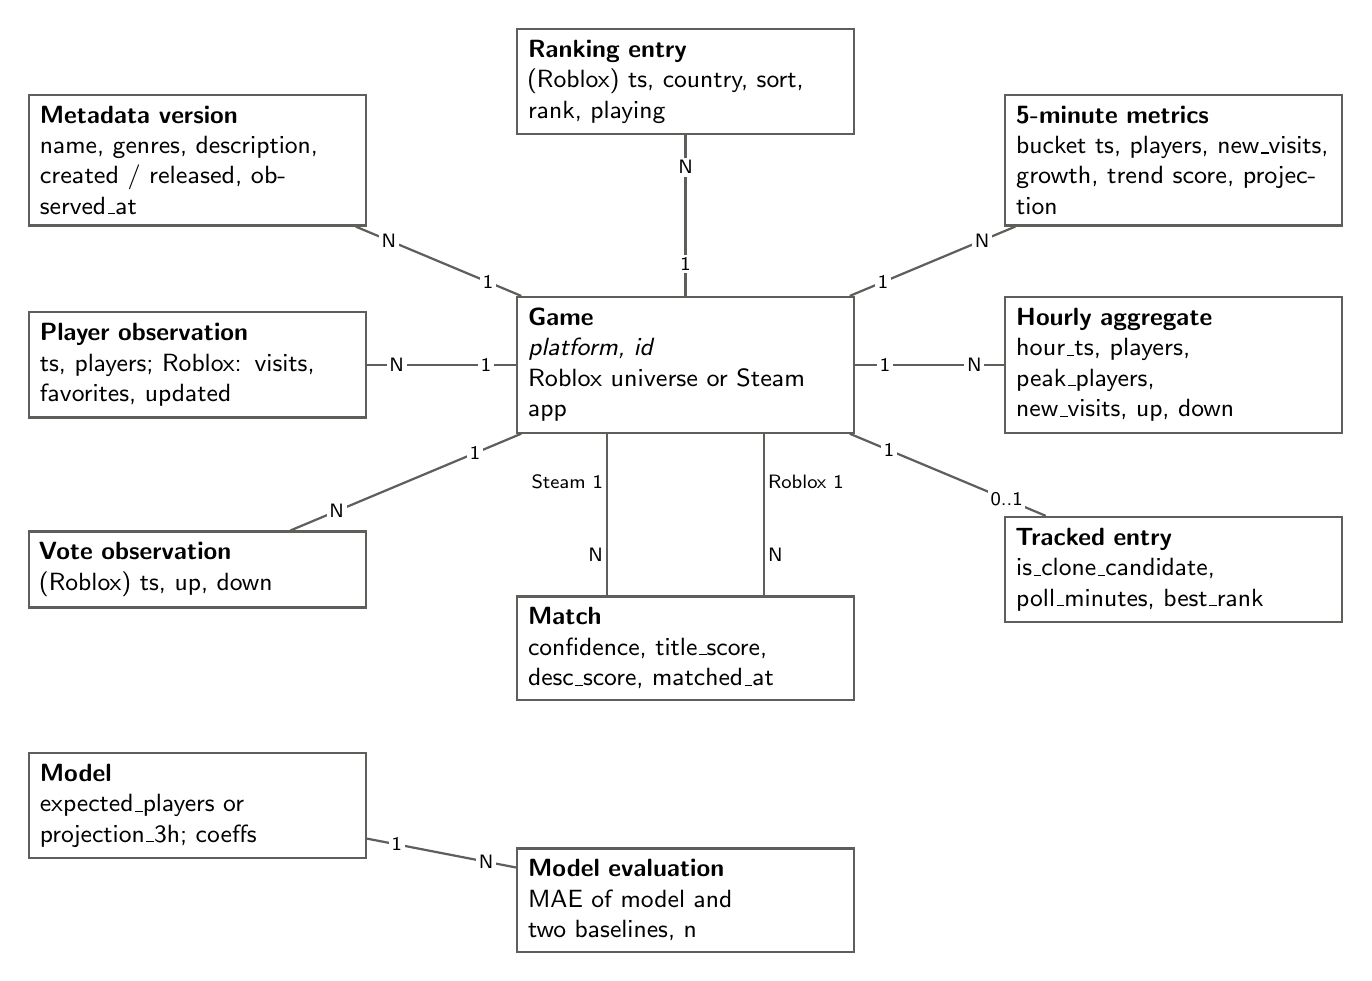
\begin{tikzpicture}[
  font=\sffamily\small,
  ent/.style={rectangle, draw=kfcgray, thick, fill=white, align=left, text width=4.0cm, inner sep=4pt},
  rel/.style={thick, draw=kfcgray},
  card/.style={font=\sffamily\scriptsize, fill=white, inner sep=1pt}
]
\node[ent] (game) at (0,0) {\textbf{Game}\\\textit{platform, id}\\Roblox universe or Steam app};
\node[ent] (meta) at (-6.2,2.6) {\textbf{Metadata version}\\name, genres, description,\\created / released, observed\_at};
\node[ent] (obs) at (-6.2,0) {\textbf{Player observation}\\ts, players; Roblox: visits,\\favorites, updated};
\node[ent] (votes) at (-6.2,-2.6) {\textbf{Vote observation}\\(Roblox) ts, up, down};
\node[ent] (sort) at (0,3.6) {\textbf{Ranking entry}\\(Roblox) ts, country, sort,\\rank, playing};
\node[ent] (m5) at (6.2,2.6) {\textbf{5-minute metrics}\\bucket ts, players, new\_visits,\\growth, trend score, projection};
\node[ent] (mh) at (6.2,0) {\textbf{Hourly aggregate}\\hour\_ts, players, peak\_players,\\new\_visits, up, down};
\node[ent] (match) at (0,-3.6) {\textbf{Match}\\confidence, title\_score,\\desc\_score, matched\_at};
\node[ent] (track) at (6.2,-2.6) {\textbf{Tracked entry}\\is\_clone\_candidate,\\poll\_minutes, best\_rank};
\node[ent] (model) at (-6.2,-5.6) {\textbf{Model}\\expected\_players or\\projection\_3h; coeffs};
\node[ent] (eval) at (0,-6.8) {\textbf{Model evaluation}\\MAE of model and\\two baselines, n};

\draw[rel] (game) -- node[card, pos=0.2]{1} node[card, pos=0.8]{N} (meta);
\draw[rel] (game) -- node[card, pos=0.2]{1} node[card, pos=0.8]{N} (obs);
\draw[rel] (game) -- node[card, pos=0.2]{1} node[card, pos=0.8]{N} (votes);
\draw[rel] (game) -- node[card, pos=0.2]{1} node[card, pos=0.8]{N} (sort);
\draw[rel] (game) -- node[card, pos=0.2]{1} node[card, pos=0.8]{N} (m5);
\draw[rel] (game) -- node[card, pos=0.2]{1} node[card, pos=0.8]{N} (mh);
\draw[rel] (game) -- node[card, pos=0.2]{1} node[card, pos=0.8]{0..1} (track);
\draw[rel] ([xshift=-1.0cm]game.south) -- node[card, pos=0.3, left]{Steam 1} node[card, pos=0.75, left]{N} ([xshift=-1.0cm]match.north);
\draw[rel] ([xshift=1.0cm]game.south) -- node[card, pos=0.3, right]{Roblox 1} node[card, pos=0.75, right]{N} ([xshift=1.0cm]match.north);
\draw[rel] (model) -- node[card, pos=0.2]{1} node[card, pos=0.8]{N} (eval);
\end{tikzpicture}
}
\caption{Conceptual data model of GameTrend Radar with relationship cardinalities.}
\label{fig:datamodel}
\end{figure}

The model maps to storage as follows. Observations are Kafka events and rows of the Parquet master dataset. Metadata versions keep only the latest version in the MongoDB collection \ep{games}. Derived entities, matches, tracked entries, models and evaluations are MongoDB collections (Section~\ref{sec:schema}).

%======================================================================
\section{Data sets}\label{sec:datasets}
Both sources are free and need no API key. The Roblox Games API is documented as a legacy API (\url{https://create.roblox.com/docs/cloud/legacy}). The Roblox discovery and search endpoints and the Steam store search are undocumented website endpoints. The Steam endpoints are documented at \url{https://partner.steamgames.com/doc/webapi/ISteamUserStats} and \url{https://partner.steamgames.com/doc/webapi/ISteamChartsService}; \ep{appdetails} is described only by the community (\url{https://wiki.teamfortress.com/wiki/User:RJackson/StorefrontAPI}).

\subsection{Recorded archive}
The collector recorded both sources from 5~Nov 2026, 19:16 to 11~Nov 2026, 17:00 (UTC), from one IP address. All responses are JSON over HTTPS, except the Steam store search, which returns HTML inside JSON. The archive keeps every HTTP attempt unchanged, including 429s, 5xx and network errors, with the request and response timestamps. Table~\ref{tab:datasets} describes each data set; the counts are means over the five full days, 6--10~Nov.

{\small
\begin{longtable}{L{2.2cm} L{2.8cm} L{1.6cm} L{2.1cm} L{6.1cm}}
\caption{Data sets. ``Records'' are game-level records, not HTTP calls.}\label{tab:datasets}\\
\toprule
\textbf{Data set} & \textbf{Category} & \textbf{Per day} & \textbf{Inflow} & \textbf{Features used (API name $\rightarrow$ event field)}\\
\midrule\endfirsthead
\toprule
\textbf{Data set} & \textbf{Category} & \textbf{Per day} & \textbf{Inflow} & \textbf{Features used}\\
\midrule\endhead
Roblox games (\eu{games.roblox.com/v1/games}) & concurrent players and cumulative counters of a Roblox game & 1.39M & one call every 3\,s, 50 IDs per call (28,800 calls/day) & \ep{playing}$\rightarrow$\ep{players}, \ep{visits}, \ep{favoritedCount}$\rightarrow$\ep{favorites}, \ep{updated}; metadata: \ep{name}, \ep{genre\_l1}, \ep{genre\_l2}, \ep{created}, \ep{description}\\
Roblox votes (\eu{/v1/games/votes}) & cumulative likes and dislikes of a game & 407k & every 5\,min per game & \ep{upVotes}$\rightarrow$\ep{up}, \ep{downVotes}$\rightarrow$\ep{down}\\
Roblox ranking lists (\eu{explore-api/v1/get-sorts}) & position of a game in the platform's ranking lists, per country (\ep{us}, \ep{br}, \ep{pl}) & 426k & every 15\,min, up to 10 pages per country & \ep{sortId}$\rightarrow$\ep{sort}, position$\rightarrow$\ep{rank}, \ep{playerCount}$\rightarrow$\ep{playing}; discovery of game IDs\\
Roblox search (\eu{search-api/omni-search}) & Roblox games whose title matches a Steam title & 131 queries & daily, one query per Steam clone candidate & \ep{universeId}, \ep{name}, \ep{playerCount} (40 results per query)\\
Steam players (\eu{GetNumberOfCurrentPlayers}) & concurrent players of a Steam game & 63k & every 5\,min per game, one game per call & \ep{player\_count}$\rightarrow$\ep{players}\\
Steam charts (\eu{GetMostPlayedGames}) & top 100 Steam games by players & 4 lists & every 6\,h & \ep{appid}, \ep{rank}, \ep{peak\_in\_game}\\
Steam new releases (\eu{store/search?filter=popularnew}) & popular new releases (clone candidates if released in the last 90 days) & 16 pages & every 6\,h, up to 5 pages of 100 & app ID, title, release date\\
Steam details (\eu{api/appdetails}) & metadata of a Steam game & 4--26 (187 on day 1) & once per new game & \ep{name}, \ep{genres}, \ep{release\_date}$\rightarrow$\ep{released}, \ep{short\_description}\\
\bottomrule
\end{longtable}}

The stream feeds deliver about 2.29M records per day, or 26.5 records per second; the Roblox games feed alone delivers 965 records per minute. The archive holds 1,641 distinct Roblox games and takes about 3.4\,GB of gzip-compressed JSON Lines, 94\,\% of it the Roblox games feed. The producers turn each record into one Kafka event and add a \ep{meta} event only when metadata changes, so Kafka receives about 2.3M events per day. The infrastructure estimate of 3M events per day assumed a 60\,s cycle for all 1,640 games; with 50 IDs per call and one call per 3\,s, a cycle over all of them takes about 100\,s.

\subsection{Data quality}\label{sec:quality}
We checked the archive for errors, gaps, missing values and suspicious values (Table~\ref{tab:quality}). The pipeline follows one rule for all of them: a missing value is an absent field, never 0 or an empty string, and 0 players is a valid observation.

\begin{table}[H]
\centering\small
\begin{tabularx}{\textwidth}{L{3.6cm} Y L{5.2cm}}
\toprule
\textbf{Issue} & \textbf{Measured in the archive} & \textbf{Handling}\\
\midrule
Failed requests & Roblox games: 11 HTTP 429 and 56 network errors in 167,021 calls (0.04\,\%); votes: 31 network errors in 49,529 calls; Steam players: 40 network errors in 382,515 calls & retried with back-off; the mock replays the recorded error windows, so the producers are tested on them\\
Collection gap & 9~Nov has about 2\,h less recording than the other full days (26,284 instead of 28,800 games calls) & the mock answers \ep{503 no-data}; growth without a reference within 15\,min stays absent\\
Steam games without player statistics & 1,672 answers (0.44\,\%) are HTTP 404 with \ep{result: 42} & no \ep{players} event; missing is not zero\\
Zero players & 177,231 of 8.2M Roblox game records (2.2\,\%) have \ep{playing = 0} & kept as valid observations; $\log(1+x)$ handles them\\
Empty descriptions & 0.4\,\% of Roblox game records; the search API returns no descriptions at all & the field is left out of \ep{meta}; matching then uses the title score alone\\
Search hits without details & only 640 of 3,119 distinct top-20 Roblox search hits (21\,\%) were also polled through \ep{/v1/games}, so the rest have no \ep{created}, \ep{description} or player history in the archive & matching scores these hits on the title alone and the dashboard shows them in grey (Section~\ref{sec:matching})\\
Repeated observations & the mock returns the same observation when polled faster than the recording & the producers skip an observation already sent\\
Duplicates after replays & producer restarts and Kafka re-reads write the same event again & Parquet keeps copies; readers drop exact copies, and the speed layer rejects older or equal observations\\
Release dates & Steam returns free text (e.g.\ ``Feb 26, 2025'', ``Q1 2027'', ``To be announced'') & converted to \ep{YYYY-MM-DD}; a value that is not a full date, or the date of an unreleased game, is left out\\
\bottomrule
\end{tabularx}
\caption{Data quality of the recorded archive.}
\label{tab:quality}
\end{table}

Two limitations remain. The archive covers about 6 days, so the models are trained once on 4 of them (Section~\ref{sec:ml}), and the ranking lists and search are undocumented endpoints that may change. The recorded responses stay in the archive, so a changed endpoint does not invalidate the data already collected.

\subsection{Input data for the regression models}\label{sec:ml-data}
Both models are regressions trained on \ep{game\_metrics\_hourly} joined with \ep{games}. Table~\ref{tab:features} defines the dependent and independent features.

{\small
\begin{longtable}{L{2.5cm} L{3.2cm} L{9.9cm}}
\caption{Features of the two regression models.}\label{tab:features}\\
\toprule
\textbf{Model} & \textbf{Feature} & \textbf{Definition}\\
\midrule\endfirsthead
\toprule
\textbf{Model} & \textbf{Feature} & \textbf{Definition}\\
\midrule\endhead
Expected players (Roblox) & dependent: $y$ & $\log(1+\text{players})$ of the game in the hour\\
 & hour of day & UTC hour of the observation, one-hot encoded\\
 & day of week & one-hot encoded\\
 & genre & \ep{genre\_l1}, one-hot encoded on the training rows; an unseen genre becomes all zeros\\
 & game age & days since \ep{created}\\
 & trailing level & mean of $\log(1+\text{players})$ over the earlier history of the game (at most 7 days), earlier observations only\\
 & like ratio & $\text{up}/(\text{up}+\text{down})$; 0.5 when votes are missing\\
\midrule
+3\,h projection (per platform) & dependent: $y_{t+3h}$ & $\log(1+\text{players})$ three hours after the current observation\\
 & current level & $\log(1+\text{players})$ now\\
 & slope & least-squares slope of $\log(1+\text{players})$ over the last 3\,h (at least 3 observations)\\
 & target hour & UTC hour of day of the target time, one-hot encoded\\
\bottomrule
\end{longtable}}

The raw data passes four transformations before training. First, the batch layer reduces the observations of a game to one per 5-minute bucket and then to one hourly document (Section~\ref{sec:transform}). Second, the player counts are log-transformed with $\log(1+x)$, because the counts span from 0 to over 400,000 and zero is valid. Third, categorical features are one-hot encoded and the encoding is saved with the coefficients, so the speed layer builds identical features. Fourth, the expected-players model excludes the game's own recent growth, since the trend score compares actual players with the expected value and would otherwise be circular. A game is scored only after 24\,h of history. The model predicts $\widehat{y}$, and the trend score is
\[
\text{trend score} = \frac{\text{players}}{\max\bigl(1, \exp(\widehat{y})-1\bigr)},
\]
where a value above 1 means more players than expected for the game's context. The projection in players is $\max(0, \exp(\widehat{y}_{t+3h})-1)$.

%======================================================================
\section{Data acquisition and transformation}\label{sec:acquisition}

\subsection{Acquisition strategy}\label{sec:acq-strategy}
Acquisition has two stages: a collector that records the live APIs, and producers that turn API responses into Kafka events. Both are Python services using \ep{requests}; the producers send to Kafka with \ep{confluent-kafka}.

\paragraph{Collector.} The collector runs six jobs, each in its own thread with its own cadence. Discovery jobs find games: the Roblox ranking lists every 15\,min, the Steam chart and new-release lists every 6\,h, and a daily Roblox search for each Steam clone candidate. Snapshot jobs poll the discovered games, at most 3,000 Roblox and 500 Steam IDs. Every response is appended unchanged to a JSON Lines file per feed and UTC hour, which is gzip-compressed when the hour closes (compression ratio 3.6 on the games feed). The collector never parses responses, so a parsing bug in a later stage can be fixed and the archive replayed.

\paragraph{API limits.} We measured the limits on 2 Nov 2026 and set one minimum interval between request starts per API group (Table~\ref{tab:limits}). Errors 429, 5xx and network errors are retried up to 6 times with exponential back-off and jitter (5\,s doubling, at most 120\,s); other statuses are final. With these intervals, 7 minutes of continuous polling gave no 429.

\begin{table}[H]
\centering\small
\begin{tabularx}{\textwidth}{L{4.0cm} L{2.0cm} Y}
\toprule
\textbf{API group} & \textbf{Interval} & \textbf{Reason}\\
\midrule
Roblox games & 3\,s & the header allows 300 req/min, but a hidden limit returns 429 after about 550 IDs in a burst\\
Roblox votes & 1\,s & header: 200 req/min; separate budget from the games API\\
Roblox ranking lists, search & 1\,s & headers: 120 req/min and 4 req/s\\
Steam Web API & 1\,s & no header; 4 req/s worked\\
Steam store & 2\,s & about 200 \ep{appdetails} requests per 5\,min\\
\bottomrule
\end{tabularx}
\caption{Minimum interval between request starts per API group.}
\label{tab:limits}
\end{table}

\paragraph{Mock API.} The mock API serves the archive over HTTP with the paths and parameters of the real endpoints. It has a replay clock $A = A_0 + (\text{wall time} - \text{start}) \cdot \text{speed}$, and it answers each request with the latest recorded observation made at or before $A$. Polling faster therefore returns the same observation again, never a later one. Every item carries its original observation time in a \ep{\_mock.observed\_at} field, and every response carries $A$ in the header \ep{X-Mock-Time}. The mock also replays the recorded error windows (429, 5xx, network errors) and can inject random errors for tests.

\paragraph{Producers.} One \ep{producers} process runs one loop per source. Every 60\,s it refreshes the list of IDs. For each stream source it sends one request every $\max(\text{pace}, \min(\text{cycle}/N, 14\,\text{s}))$ seconds, where $N$ is the number of requests in one round over all IDs. With 1,155 Roblox IDs that is one games request every 3\,s and one votes request every 12.5\,s. Each request starts on schedule, without waiting for the previous answer, with a 10\,s timeout. The producers then:
\begin{enumerate}
  \item parse each response into events of the Kafka contract (Section~\ref{sec:schema}) and keep only the listed fields;
  \item take the event time \ep{ts} from \ep{\_mock.observed\_at} on the mock, or from the request time on the live APIs;
  \item drop events whose \ep{ts} is later than \ep{X-Mock-Time}, because one future timestamp would move every data-time cutoff downstream;
  \item skip an observation already sent (same \ep{observed\_at} per endpoint and ID) and send a \ep{meta} event only when the metadata changed;
  \item validate every event with the shared contract check and drop and count the invalid ones;
  \item send the event keyed by game ID, with the \ep{murmur2\_random} partitioner, so all events of a game land in one partition as with the Java clients.
\end{enumerate}
The producers count requests, sent, dropped, failed and erroneous records per feed and log the counts every minute. Writing these counters to \ep{ingest\_stats} is planned.

\subsection{Transformation steps}\label{sec:transform}
Events pass three transformation paths after Kafka, one per consumer.

\paragraph{Speed layer.} One Spark Structured Streaming query reads both topics and hands each micro-batch (at most 50,000 records) to Python code in \ep{foreachBatch}. The code validates each record with the same contract check as the producers and groups observations into 5-minute buckets per game. Within a bucket the latest observation wins; ties are decided by the values, never by arrival order. It then computes \ep{new\_visits} (the visit delta to the previous bucket, absent after a counter reset or a gap over 1\,h) and the growth over 1\,h, 3\,h and 24\,h. The growth reference is the observation nearest to the current time minus the horizon, at most 15\,min away. History comes from one MongoDB query per platform and micro-batch. Writes are conditional upserts: a write matches only if the stored \ep{observed\_at} is older, so a replayed or late event never overwrites newer data. Trend score and projection are planned, because the models do not exist yet.

\paragraph{Parquet sink.} The batch layer archives every valid event of both topics in the master dataset. The sink is a Structured Streaming query with the \ep{availableNow} trigger: each hourly cycle archives what Kafka holds at its start and stops. Records are validated with the shared contract check and converted to rows inside \ep{mapInPandas}, with nullable integer columns so a missing value never becomes 0. The Parquet columns are derived from the contract check's schema, so the contract is defined once.

\paragraph{Hourly aggregates and retention.} Each cycle computes the closed hours from the master dataset, starting two hours before the latest hour already in MongoDB, so late events of the last two hours are included. Exact copies are dropped first; then each game is aggregated with \ep{applyInPandas}, using the same metric functions as the speed layer, so live and hourly numbers agree. Each hour is written in one MongoDB transaction, so the dashboard never reads a half-written hour. After the aggregates succeed, a retention sweep deletes 5-minute documents older than 14 days, but only for games that have an hourly document for that hour. ``Now'' for the cutoff is the latest event time in Parquet.

\subsection{Storage strategy}\label{sec:storage}
Each store holds one view of the data for a fixed time (Table~\ref{tab:storage}). Kafka is the buffer between acquisition and processing. Parquet is the immutable master dataset from which every derived value can be recomputed. MongoDB holds only what the dashboard and the speed layer read.

\begin{table}[H]
\centering\small
\begin{tabularx}{\textwidth}{L{3.2cm} L{4.0cm} Y L{2.4cm}}
\toprule
\textbf{Store} & \textbf{Format} & \textbf{Content and layout} & \textbf{Retention}\\
\midrule
Raw archive & JSON Lines, gzip, per feed and UTC hour & every HTTP attempt, unchanged & whole project\\
Kafka 3.7 & JSON, key = game ID & topic \ep{roblox.snapshots} (3 partitions), \ep{steam.players} (1 partition); broker time as record timestamp, so old replayed events do not expire at once & 72--96\,h\\
Parquet master dataset & Parquet, Snappy & one wide table of all events, partitioned by \ep{platform} and UTC \ep{date} of \ep{ts}; append-only, copies kept and removed by readers & whole project\\
MongoDB 7 & BSON documents, unique compound index per collection & 5-minute metrics, hourly aggregates, metadata, matches, models & 14 days (5-min), whole project (rest)\\
\bottomrule
\end{tabularx}
\caption{Storage layers.}
\label{tab:storage}
\end{table}

\subsection{Data schema}\label{sec:schema}
\paragraph{Kafka topics.} The topic \ep{roblox.snapshots} carries the kinds \ep{game}, \ep{votes}, \ep{sort} and \ep{meta}, and \ep{steam.players} carries \ep{players} and \ep{meta}; their fields are the event fields in Table~\ref{tab:datasets}. Every event also has \ep{kind}, \ep{ts} (ISO-8601 UTC) and \ep{id}. Every field is required, except in \ep{meta} events, where only \ep{name} is required.

\paragraph{MongoDB collections.} Each collection has a unique compound index on its key fields, and every write is an upsert on that key.

{\small
\begin{longtable}{L{3.0cm} L{9.6cm} L{2.9cm}}
\toprule
\textbf{Collection} & \textbf{Main fields} & \textbf{Written by}\\
\midrule\endhead
\ep{game\_metrics} & key \ep{platform, id, ts}; \ep{observed\_at, votes\_observed\_at, players, visits, new\_visits, favorites, updated, up, down, growth\_1h, growth\_3h, growth\_24h, trend\_score, projection\_3h} & speed (5\,min), batch (deletes)\\
\ep{game\_metrics\_hourly} & key \ep{platform, id, hour\_ts}; \ep{players, peak\_players, new\_visits, updated, up, down} & batch (hourly)\\
\ep{games} & key \ep{platform, id}; \ep{name, genre\_l1, genre\_l2, genres, description, created, released, observed\_at} & speed\\
\ep{tracked\_games} & key \ep{platform, id}; \ep{is\_clone\_candidate, poll\_minutes, best\_rank} (new: best ranking-list position of the last 7 days) & batch (daily)\\
\ep{bv\_matches} & key \ep{steam\_id, roblox\_id}; \ep{confidence, title\_score, desc\_score, matched\_at}; new for untracked hits: \ep{roblox\_name, search\_players} (name and player count from the search result) & matching (daily)\\
\ep{model\_coeffs} & key \ep{model, platform, trained\_at}; \ep{coeffs, preprocessing, r2, rmse} & ml (once)\\
\ep{model\_health} & key \ep{platform, evaluated\_at}; \ep{mae\_model, mae\_now, mae\_yesterday, n} & ml (once)\\
\ep{ingest\_stats} & key \ep{feed, ts}; \ep{ok, dropped, errors} & producers\\
\bottomrule
\end{longtable}}

%======================================================================
\section{System architecture}\label{sec:architecture}
GameTrend Radar follows the lambda architecture (Figure~\ref{fig:architecture}). Kafka feeds two independent paths. The speed layer updates 5-minute metrics within one micro-batch. The batch layer archives every event in an immutable master dataset and recomputes hourly aggregates from it. Both paths write to the serving layer, MongoDB, which the dashboard reads. Kafka keeps events for 72--96\,h, so any reprocessing of older history reads the Parquet master dataset, not Kafka; the hourly aggregates and the planned one-time model training both read days of history from it.

\begin{landscape}
\begin{figure}[p]
\centering
\resizebox{\linewidth}{!}{% Solution architecture (lambda). Implemented: solid border, tinted fill. Planned (next phases): dashed border, white fill, PLANNED tag.
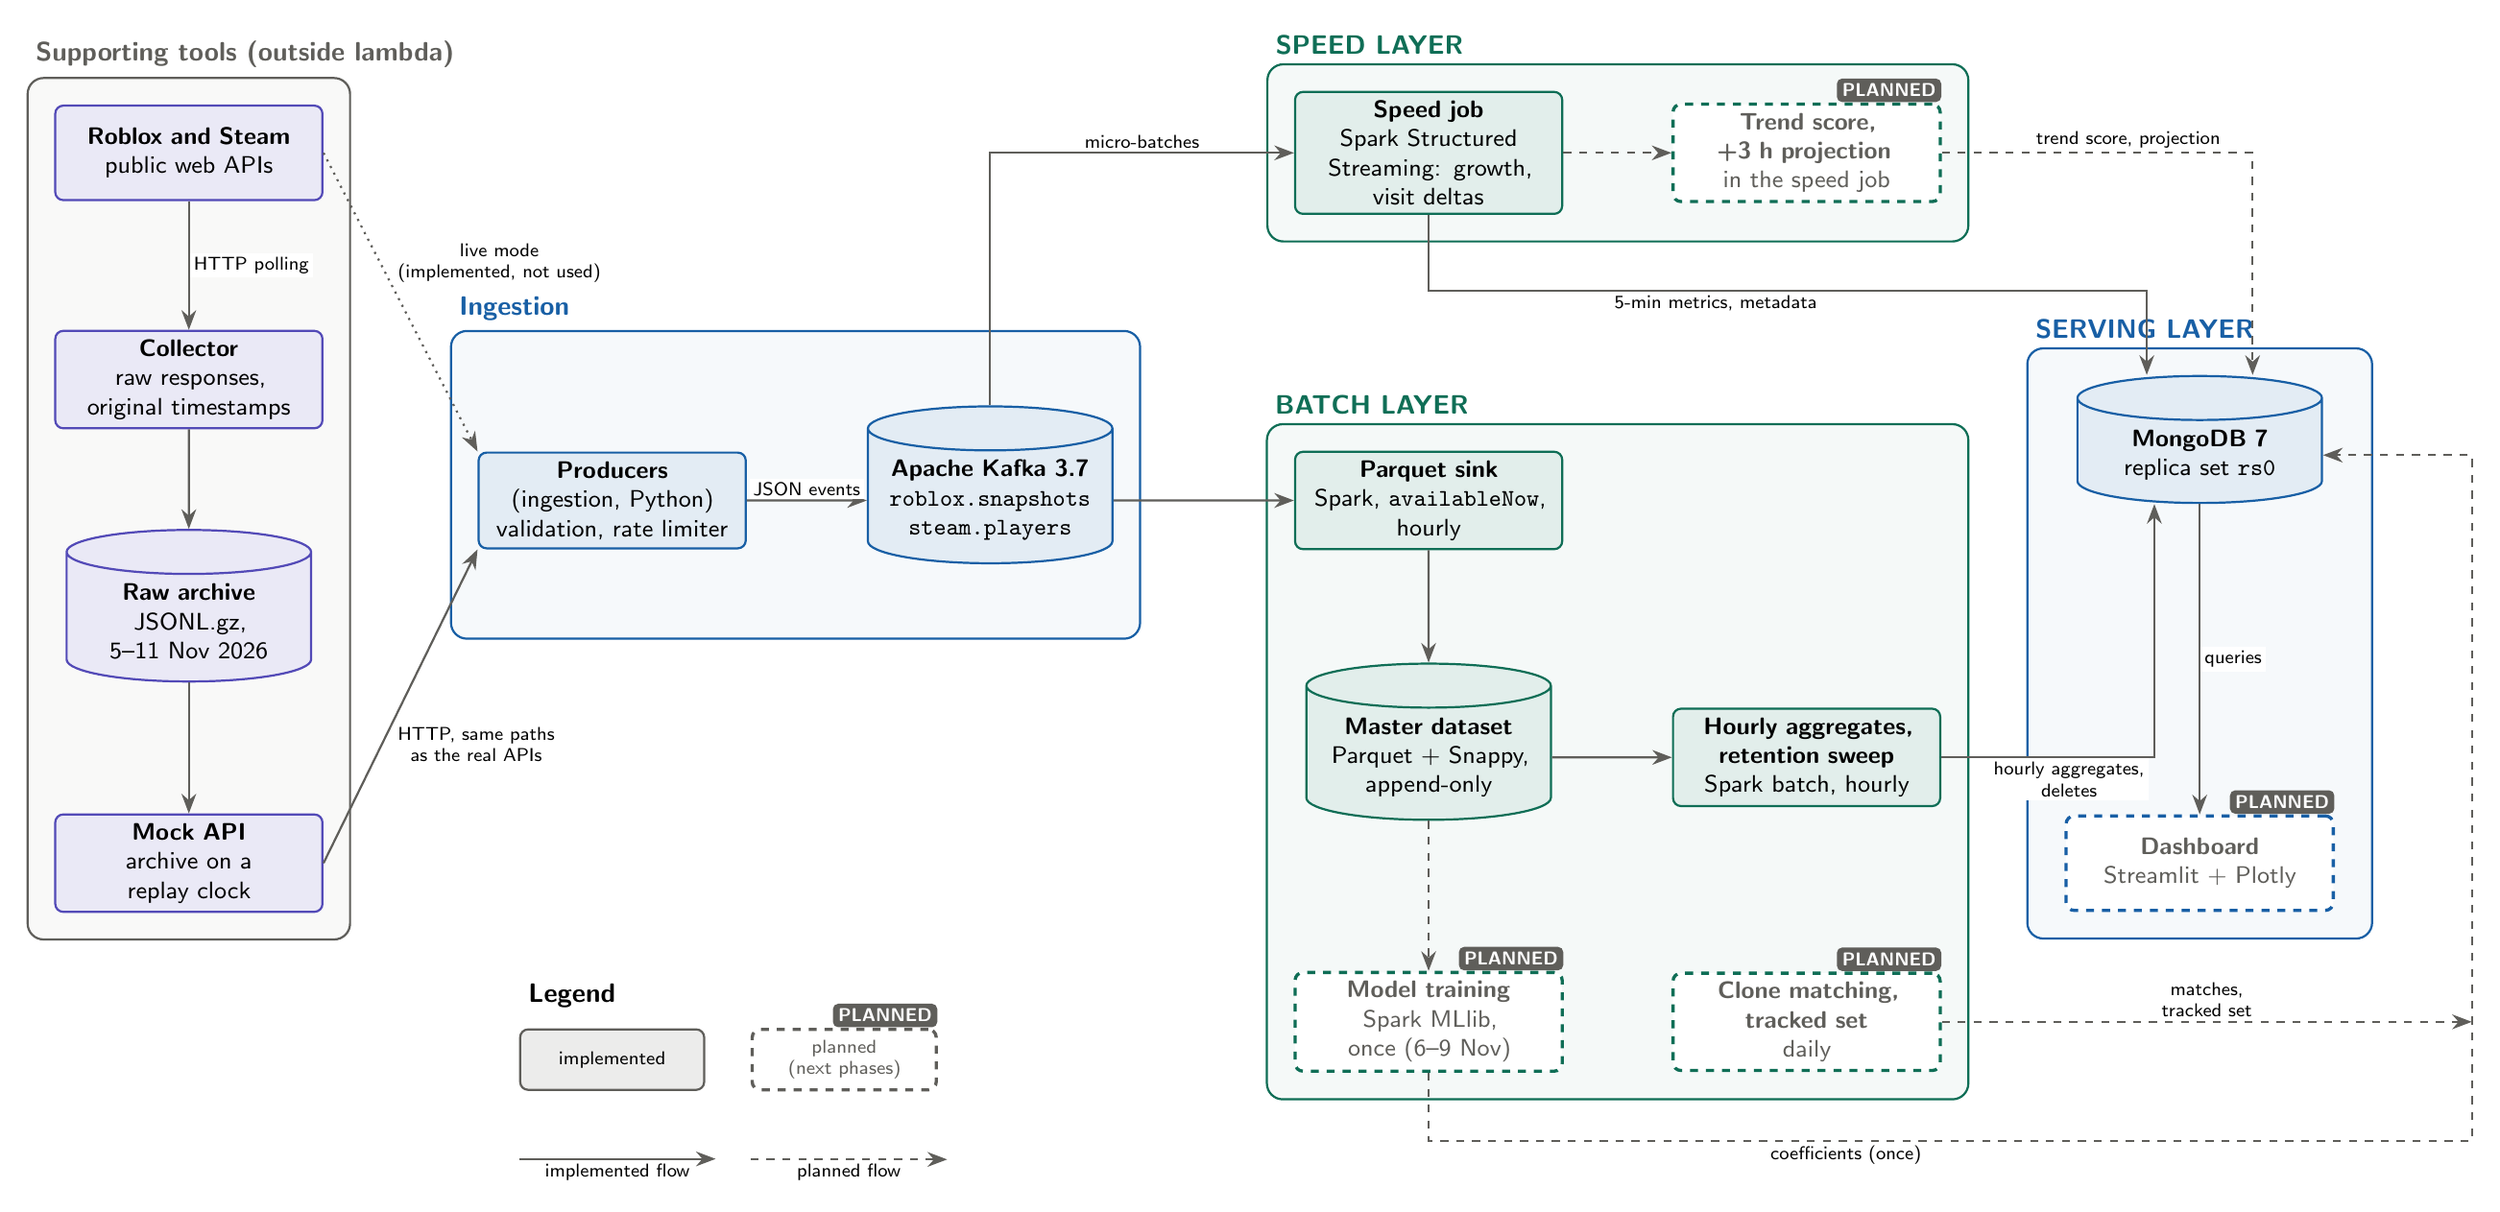
\begin{tikzpicture}[
  font=\sffamily\small,
  box/.style={rectangle, rounded corners=3pt, draw=#1, fill=#1!12, thick, align=center, minimum height=1.25cm, text width=3.3cm},
  box/.default=kfcgray,
  db/.style={cylinder, shape border rotate=90, aspect=0.18, draw=#1, fill=#1!12, thick, align=center, minimum height=1.45cm, text width=3.0cm},
  db/.default=kfcgray,
  plan/.style={dashed, fill=white, text=kfcgray, line width=1.2pt},
  tag/.style={font=\sffamily\scriptsize\bfseries, text=white, fill=kfcgray, rounded corners=2pt, inner sep=2pt, anchor=south east},
  arr/.style={-{Stealth[length=2.6mm]}, thick, draw=kfcgray},
  parr/.style={arr, dashed},
  altarr/.style={arr, dotted},
  lab/.style={font=\sffamily\scriptsize, fill=white, inner sep=1.5pt, align=center},
  layer/.style={rectangle, rounded corners=6pt, draw=#1, fill=#1!4, thick, inner sep=10pt},
  ltitle/.style={font=\sffamily\bfseries, text=#1, anchor=south west}
]
% ---------------- sources and supporting tools
\node[box=kfcpurple] (api) at (0,4.6) {\textbf{Roblox and Steam}\\public web APIs};
\node[box=kfcpurple] (coll) at (0,1.6) {\textbf{Collector}\\raw responses,\\original timestamps};
\node[db=kfcpurple] (raw) at (0,-1.6) {\textbf{Raw archive}\\JSONL.gz,\\5--11 Nov 2026};
\node[box=kfcpurple] (mock) at (0,-4.8) {\textbf{Mock API}\\archive on a\\replay clock};
% ---------------- ingestion
\node[box=kfcblue] (prod) at (5.6,0) {\textbf{Producers}\\(ingestion, Python)\\validation, rate limiter};
\node[db=kfcblue] (kafka) at (10.6,0) {\textbf{Apache Kafka 3.7}\\\texttt{roblox.snapshots}\\\texttt{steam.players}};
% ---------------- speed layer
\node[box=kfcteal] (speed) at (16.4,4.6) {\textbf{Speed job}\\Spark Structured\\Streaming: growth,\\visit deltas};
\node[box=kfcteal, plan] (score) at (21.4,4.6) {\textbf{Trend score,}\\\textbf{+3 h projection}\\in the speed job};
% ---------------- batch layer
\node[box=kfcteal] (sink) at (16.4,0) {\textbf{Parquet sink}\\Spark, \texttt{availableNow},\\hourly};
\node[db=kfcteal] (master) at (16.4,-3.4) {\textbf{Master dataset}\\Parquet + Snappy,\\append-only};
\node[box=kfcteal] (agg) at (21.4,-3.4) {\textbf{Hourly aggregates,}\\\textbf{retention sweep}\\Spark batch, hourly};
\node[box=kfcteal, plan] (train) at (16.4,-6.9) {\textbf{Model training}\\Spark MLlib,\\once (6--9 Nov)};
\node[box=kfcteal, plan] (match) at (21.4,-6.9) {\textbf{Clone matching,}\\\textbf{tracked set}\\daily};
% ---------------- serving layer
\node[db=kfcblue] (mongo) at (26.6,0.6) {\textbf{MongoDB 7}\\replica set \texttt{rs0}};
\node[box=kfcblue, plan] (dash) at (26.6,-4.8) {\textbf{Dashboard}\\Streamlit + Plotly};

% PLANNED tags
\foreach \n in {score, train, match, dash} {\node[tag] at (\n.north east) {PLANNED};}

% ---------------- layers
\begin{scope}[on background layer]
  \node[layer=kfcgray, fit=(api)(coll)(raw)(mock), label={[ltitle=kfcgray]north west:Supporting tools (outside lambda)}] {};
  \node[layer=kfcblue, fit=(prod)(kafka), inner ysep=28pt, label={[ltitle=kfcblue]north west:Ingestion}] {};
  \node[layer=kfcteal, fit=(speed)(score), label={[ltitle=kfcteal]north west:SPEED LAYER}] {};
  \node[layer=kfcteal, fit=(sink)(master)(agg)(train)(match), label={[ltitle=kfcteal]north west:BATCH LAYER}] {};
  \node[layer=kfcblue, fit=(mongo)(dash), inner xsep=14pt, label={[ltitle=kfcblue]north west:SERVING LAYER}] {};
\end{scope}

% ---------------- flows
\draw[arr] (api) -- node[lab, right]{HTTP polling} (coll);
\draw[arr] (coll) -- (raw);
\draw[arr] (raw) -- (mock);
\draw[arr] (mock.east) -- node[lab, pos=0.45, below right]{HTTP, same paths\\as the real APIs} (prod.south west);
\draw[altarr] (api.east) -- node[lab, pos=0.45, above right]{live mode\\(implemented, not used)} (prod.north west);
\draw[arr] (prod) -- node[lab, above]{JSON events} (kafka);
\draw[arr] (kafka.north) |- node[lab, pos=0.75, above]{micro-batches} (speed.west);
\draw[arr] (kafka.east) -- (sink.west);
\draw[parr] (speed) -- (score);
\draw[arr] (sink) -- (master);
\draw[arr] (master) -- (agg);
\draw[parr] (master) -- (train);
\draw[arr] (speed.south) |- ++(0,-1.0) -| node[lab, pos=0.2, below]{5-min metrics, metadata} ([xshift=-0.7cm]mongo.north);
\draw[parr] (score.east) -| node[lab, pos=0.3, above]{trend score, projection} ([xshift=0.7cm]mongo.north);
\draw[arr] (agg.east) -| node[lab, pos=0.3, below]{hourly aggregates,\\deletes} ([xshift=-0.6cm]mongo.south);
\draw[parr] (train.south) -- ++(0,-0.9) -| node[lab, pos=0.2, below]{coefficients (once)} (30.2,-1) |- (mongo.east);
\draw[parr] (match.east) -- node[lab, above]{matches,\\tracked set} (30.2,-6.9);
\draw[arr] (mongo) -- node[lab, right]{queries} (dash);

% ---------------- legend
\node[box, text width=2.2cm, minimum height=0.8cm, font=\sffamily\scriptsize] (l1) at (5.6,-7.4) {implemented};
\node[box, plan, text width=2.2cm, minimum height=0.8cm, font=\sffamily\scriptsize, right=0.6cm of l1] (l2) {planned (next phases)};
\node[tag] at (l2.north east) {PLANNED};
\draw[arr] ([yshift=-0.9cm]l1.south west) -- node[lab, below]{implemented flow} ++(2.6,0);
\draw[parr] ([yshift=-0.9cm]l2.south west) -- node[lab, below]{planned flow} ++(2.6,0);
\node[font=\sffamily\bfseries, anchor=south west] at ([yshift=0.15cm]l1.north west) {Legend};
\end{tikzpicture}
}
\caption{Solution architecture with the lambda layers marked: solid, tinted boxes and arrows are implemented, dashed boxes with a PLANNED tag and dashed arrows are planned for the next phases, and the dotted arrow is the implemented but unused live mode.}
\label{fig:architecture}
\end{figure}
\end{landscape}

\paragraph{Data flows.} Acquisition, the speed path and the batch path follow the arrows of Figure~\ref{fig:architecture}; their transformation steps are in Section~\ref{sec:transform}. The dashboard reads only MongoDB. A shared history read will take each hour from the 5-minute documents if they still exist and from the hourly document otherwise, so a chart has neither gaps nor double counts at the 14-day retention boundary.

\paragraph{Consistency between layers.} The speed and batch layers call the same Python functions for buckets, growth and visit deltas, so a value computed live equals the value recomputed in batch for the same input. The hourly value from batch is authoritative: the speed layer computes visit deltas in arrival order, and a bucket that arrives after a later bucket of the same game makes its live delta too high. In normal operation this does not happen, since all events of a game share one Kafka partition.

\paragraph{Failure handling.} The speed job fails fast on any MongoDB error other than a rejected older write, and Docker restarts it up to 5 times; Spark repeats the micro-batch from the checkpoint, and the guarded upserts make the repeat harmless. The batch loop isolates its steps: a failing aggregate step does not stop archiving, because Kafka keeps events only 72\,h while aggregates can always be recomputed. A sink outage shorter than 72\,h loses no data.

\paragraph{Deployment.} Everything runs on one computer with Docker Compose. Kafka runs as one KRaft broker (\ep{apache/kafka:3.7.0}, 1\,GB) and MongoDB as a single-node replica set (\ep{mongo:7.0.16}, 1\,GB), which the multi-document transactions of the batch layer require. Init containers create the Kafka topics and the MongoDB indexes from the contracts at every start. Spark runs in local mode: \ep{speed} (2\,GB) and \ep{batch} (2.5\,GB) are separate containers of one image, \ep{gametrend-spark:dev}, each with driver and executors in one JVM. The collector, the mock API and the producers run as Python 3.11 processes on the host. Table~\ref{tab:tech} lists the technologies of every layer.

\begin{table}[H]
\centering\small
\begin{tabularx}{\textwidth}{L{3.0cm} Y}
\toprule
\textbf{Layer} & \textbf{Technology}\\
\midrule
Acquisition & Python 3.11, \ep{requests}, raw archive in JSON Lines + gzip, mock API on the standard-library HTTP server\\
Messaging & Apache Kafka 3.7 (KRaft, one broker), \ep{confluent-kafka}\\
Batch storage & Parquet + Snappy on a Docker volume\\
Stream processing & Spark 3.5 Structured Streaming (PySpark, local mode), \ep{pymongo}\\
Batch processing & Spark 3.5 batch with \ep{mapInPandas}/\ep{applyInPandas}, pandas\\
Machine learning & Spark MLlib linear regression\\
Clone matching & \ep{rapidfuzz} (titles), \ep{scikit-learn} TF--IDF (descriptions)\\
Serving & MongoDB 7 (single-node replica set)\\
Presentation & Streamlit + Plotly\\
Orchestration & Docker Compose; \ep{batch} loop with a fixed pause\\
\bottomrule
\end{tabularx}
\caption{Technologies by layer; Section~\ref{sec:status} gives the implementation status of each area.}
\label{tab:tech}
\end{table}

%======================================================================
\section{Analytical approach}\label{sec:analytics}
We plan five analytical tasks. Table~\ref{tab:tasks} shows for each the task type and the role of batch and stream processing. The pattern is the same for both models: the batch layer trains on hourly history, and the speed layer applies the latest coefficients to every 5-minute document.

{\small
\begin{longtable}{L{2.8cm} L{2.6cm} L{5.0cm} L{4.6cm}}
\caption{Analytical tasks and their use of batch and stream processing.}\label{tab:tasks}\\
\toprule
\textbf{Task} & \textbf{Type} & \textbf{Batch processing} & \textbf{Stream processing}\\
\midrule\endfirsthead
\toprule
\textbf{Task} & \textbf{Type} & \textbf{Batch processing} & \textbf{Stream processing}\\
\midrule\endhead
Growth and visits & descriptive metrics & authoritative hourly values from Parquet (implemented) & 1\,h/3\,h/24\,h growth and visit deltas per 5-min bucket (implemented)\\
Trend score & regression (expected players) & one training on 6--9~Nov, evaluation on 10~Nov with $R^2$ and RMSE & score = actual / expected players for each Roblox document\\
+3\,h projection & regression (short-term forecast) & one training per platform on the same slice; MAE on 10~Nov against ``same as now'' and ``same time yesterday'' & projection for each 5-min document\\
Clone matching & entity matching by text similarity & daily: search, scoring, \ep{bv\_matches} rebuild & none\\
Saturation & aggregation & daily or at query time (open) & latest players of the matched games\\
\bottomrule
\end{longtable}}

\subsection{Models}\label{sec:ml}
Both models are Spark MLlib linear regressions trained once on the hourly aggregates of a fixed slice of the archive, 6--9~Nov (4 full days). After this one training run, the models are deployed and never retrained: no scheduled training job exists. The archive holds about 6 days, and one fixed model is enough to compute the trend score and the projection on the replayed stream. The training job saves the coefficients together with the preprocessing (for example the genre levels of the one-hot encoding) in \ep{model\_coeffs}, and the speed layer reads them at the start of each micro-batch. The features are defined in Table~\ref{tab:features}.

Both models are evaluated once on the following full day, 10~Nov, which the training never sees. The expected-players model reports $R^2$, RMSE in players and the sample count. For the projection, the target of every 5-minute document of that day is the actual player count 3\,h later; we compare the MAE of the model with the MAE of two baselines on exactly the same targets: \emph{same as now} (current players) and \emph{same time yesterday} (players 24\,h before the target). A projection that does not beat the first baseline adds no value, and the health page will show it. The cost of a fixed model is that it does not adapt to trends after 9~Nov.

\subsection{Clone matching}\label{sec:matching}
Once a day, the matching job takes the top 10--20 Roblox search hits for the title of every Steam clone candidate. It normalises the titles (emoji, bracketed tags such as ``[UPD 3]'' and punctuation removed, lower case). The Steam title, description and release date come from \ep{appdetails} (172 of 175 candidates have them), and the search results come from the archive. The job scores every hit, but the input differs between two kinds of hits. A tracked hit, that is a Roblox game we poll, has \ep{created} and a description in \ep{games}, so the job keeps it only if it was created after the Steam release and scores it on title and description. An untracked hit has neither, so the job scores it on the title alone and cannot apply the date rule. The match confidence is
\[
\text{confidence} = 0.5 \cdot s_{\text{title}} + 0.5 \cdot s_{\text{desc}},
\]
where $s_{\text{title}}$ is the fuzzy token-set ratio of the titles and $s_{\text{desc}}$ is the TF--IDF cosine similarity of the descriptions; if either description is empty, the confidence is $s_{\text{title}}$. Pairs above one fixed threshold go to \ep{bv\_matches}. Untracked matches have more false positives, because an older Roblox game with a similar title passes without the date rule. The team will label about 100 candidate pairs and report precision separately for tracked and untracked matches. All of this works on the recorded archive; no data has to be fetched again.

\subsection{Presentation of results}\label{sec:presentation}
The dashboard (Streamlit + Plotly, planned) presents the results in four views.
\begin{itemize}
  \item \emph{Trending now} (entry point): Roblox games ranked by trend score and Steam games ranked by growth, with current players and the +3\,h projection, filtered by genre.
  \item \emph{Game details}: metrics and a player time series (5-minute data for the last 14 days, hourly data beyond) with update markers and the projection. A Roblox game lists its possible Steam counterparts as links. A Steam game shows its growth, its saturation and the table of its possible Roblox counterparts.
  \item \emph{Steam$\rightarrow$Roblox opportunities} (supplementary): Steam games released in the last 90 days with 1\,h/3\,h/24\,h growth, their matched Roblox games with confidence, and saturation (number of matched games and their total players).
  \item \emph{Model and data health}: projection MAE against both baselines per platform, data freshness per feed and API errors.
\end{itemize}
The core use case navigates through three screens (Figure~\ref{fig:wire}): from \emph{Trending now} to the details of a Roblox game, from there to one of its possible Steam counterparts, and from the Steam game back to any tracked Roblox counterpart. Every table of possible Roblox counterparts shows two kinds of rows. A tracked game carries a badge with its best position in the ranking lists of the last 7 days and opens its full details. An untracked game is shown in grey, with the player count from the search result and a note that it is a single reading; it has no history. Saturation counts both kinds and states how many matched games are untracked. The dashboard shows a missing value as unavailable, never as zero, and labels matches as \emph{possible counterparts}, since the heuristic does not verify copying. A Roblox game gets a trend score only after 24\,h of history. \emph{Trending now} lists the scored games first, by trend score, and the games without a score below them, by \ep{growth\_1h}; a game without either is listed last.

\begin{figure}[H]
\centering
\resizebox{\textwidth}{!}{% Wireframe of the core use case: Trending now -> Roblox game details -> Steam game details.
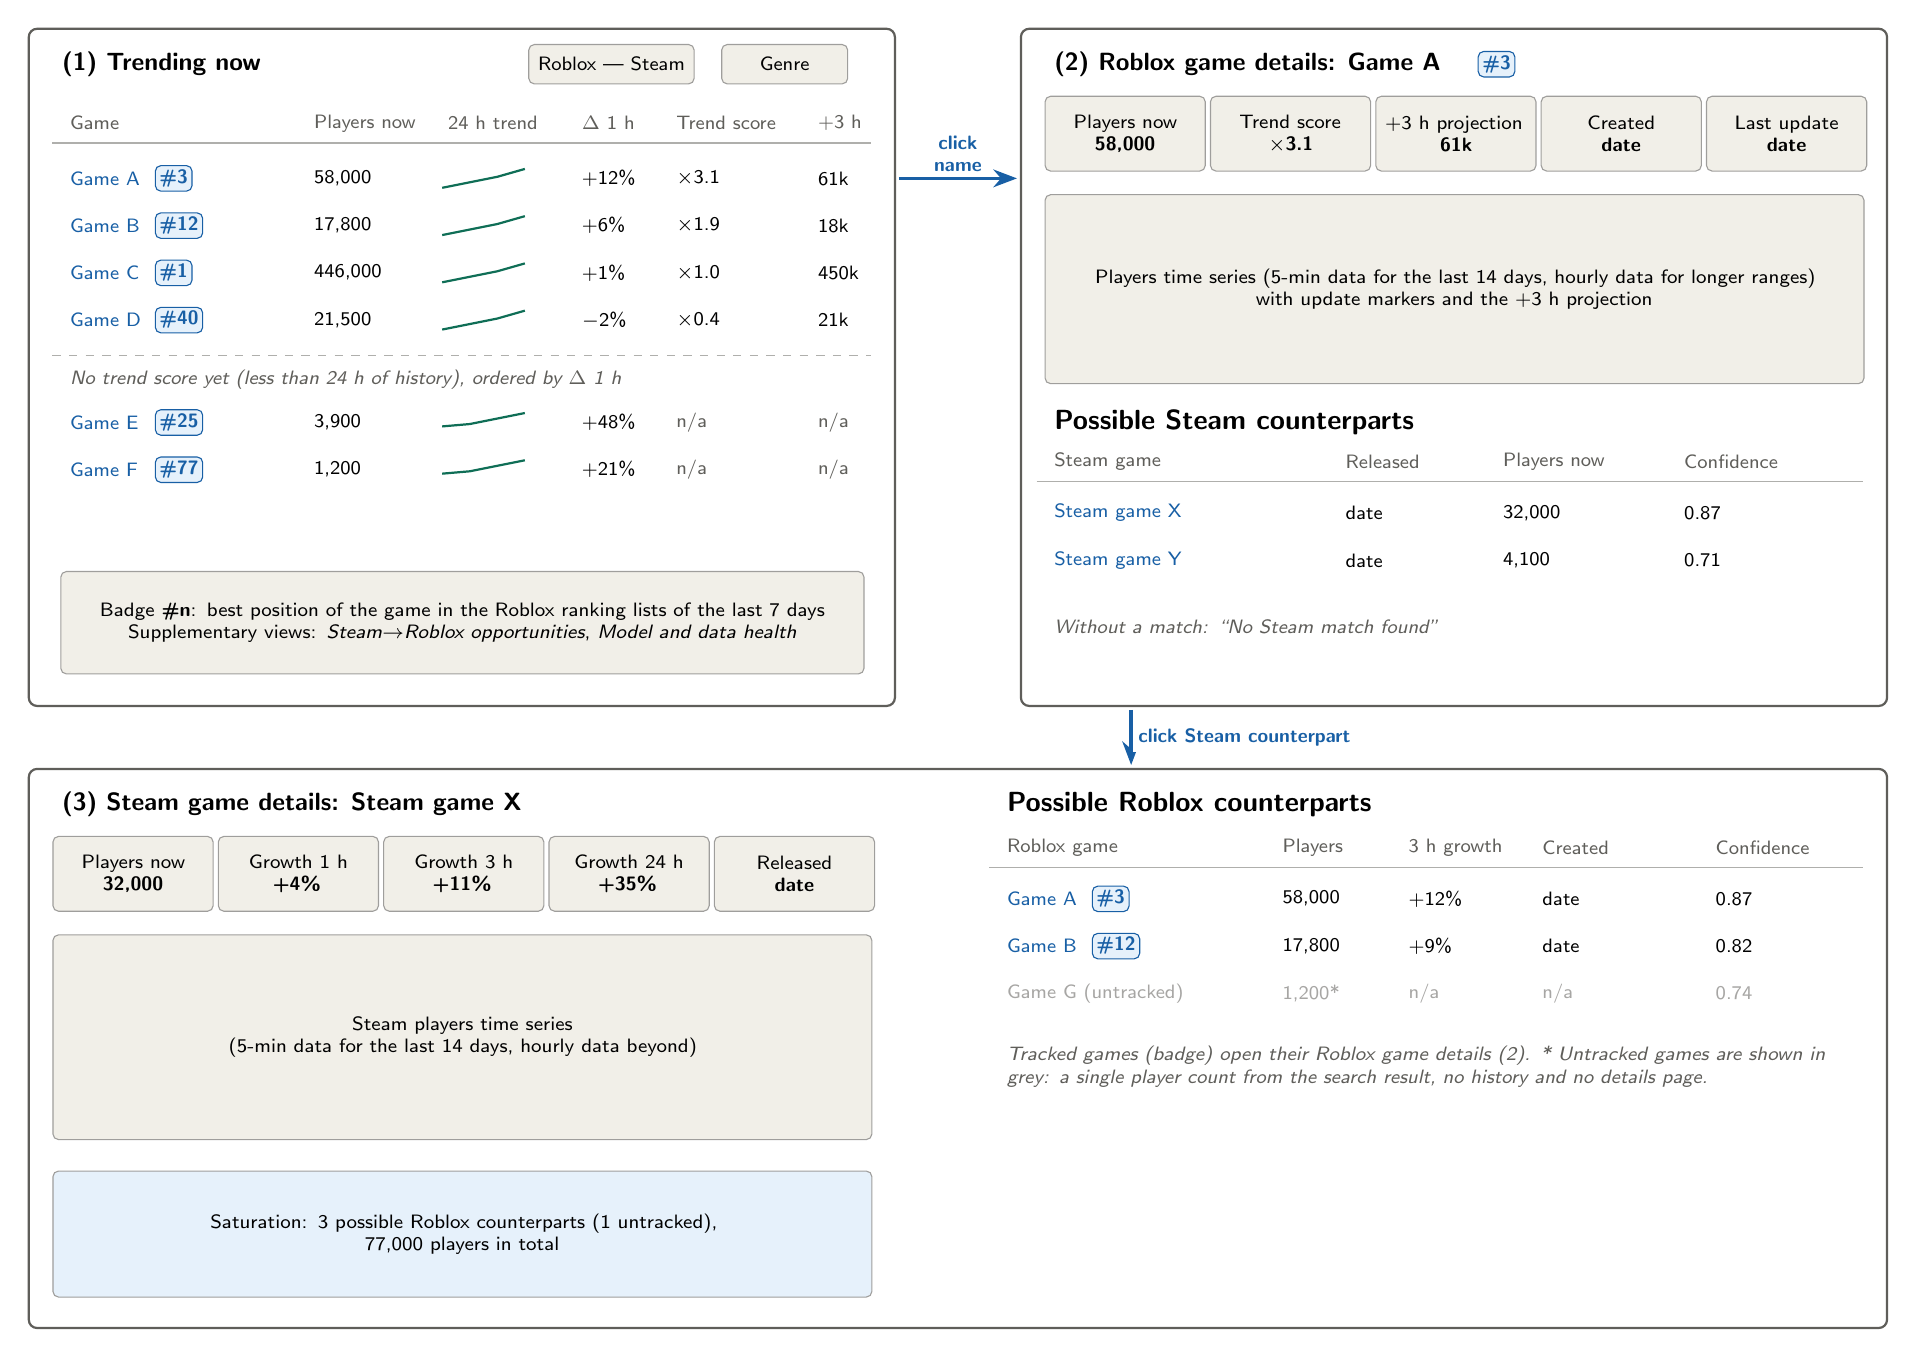
\begin{tikzpicture}[font=\sffamily\scriptsize,
  frame/.style={draw=kfcgray, thick, rounded corners=3pt},
  ph/.style={draw=kfcgray!60, fill=lightgray, rounded corners=2pt, align=center},
  hd/.style={font=\sffamily\bfseries\small},
  badge/.style={draw=kfcblue, fill=lightblue, text=kfcblue, rounded corners=2pt, inner sep=1.5pt, font=\sffamily\scriptsize\bfseries},
  grey/.style={text=kfcgray!55},
  link/.style={text=kfcblue},
  nav/.style={-{Stealth[length=3mm]}, very thick, draw=kfcblue},
  navlab/.style={font=\sffamily\scriptsize\bfseries, text=kfcblue, fill=white, inner sep=2pt}]
% ================= (1) Trending now
\draw[frame] (0,0) rectangle (11,8.6);
\node[hd, anchor=west] at (0.3,8.15) {(1) Trending now};
\node[ph, minimum width=1.9cm, minimum height=0.5cm] at (7.4,8.15) {Roblox | Steam};
\node[ph, minimum width=1.6cm, minimum height=0.5cm] at (9.6,8.15) {Genre};
\foreach \xx/\tx in {0.4/Game, 3.5/Players now, 5.2/24 h trend, 6.9/$\Delta$ 1 h, 8.1/Trend score, 9.9/+3 h} {\node[anchor=west, text=kfcgray] at (\xx,7.4) {\tx};}
\draw[kfcgray!50] (0.3,7.15) -- (10.7,7.15);
\foreach \yy/\nm/\rk/\pc/\dl/\sc/\pr in {6.7/Game A/\#3/58{,}000/+12\%/$\times$3.1/61k, 6.1/Game B/\#12/17{,}800/+6\%/$\times$1.9/18k, 5.5/Game C/\#1/446{,}000/+1\%/$\times$1.0/450k, 4.9/Game D/\#40/21{,}500/$-$2\%/$\times$0.4/21k} {
  \node[anchor=west, link] at (0.4,\yy) {\nm}; \node[badge, anchor=west] at (1.6,\yy) {\rk};
  \node[anchor=west] at (3.5,\yy) {\pc};
  \draw[kfcteal, thick] (5.25,\yy-0.12) -- (5.6,\yy-0.05) -- (5.95,\yy+0.02) -- (6.3,\yy+0.12);
  \node[anchor=west] at (6.9,\yy) {\dl}; \node[anchor=west] at (8.1,\yy) {\sc}; \node[anchor=west] at (9.9,\yy) {\pr};}
\draw[kfcgray!50, dashed] (0.3,4.45) -- (10.7,4.45);
\node[anchor=west, text=kfcgray, font=\sffamily\scriptsize\itshape] at (0.4,4.15) {No trend score yet (less than 24 h of history), ordered by $\Delta$ 1 h};
\foreach \yy/\nm/\rk/\pc/\dl in {3.6/Game E/\#25/3{,}900/+48\%, 3.0/Game F/\#77/1{,}200/+21\%} {
  \node[anchor=west, link] at (0.4,\yy) {\nm}; \node[badge, anchor=west] at (1.6,\yy) {\rk};
  \node[anchor=west] at (3.5,\yy) {\pc};
  \draw[kfcteal, thick] (5.25,\yy-0.05) -- (5.6,\yy-0.02) -- (5.95,\yy+0.05) -- (6.3,\yy+0.12);
  \node[anchor=west] at (6.9,\yy) {\dl}; \node[anchor=west, text=kfcgray] at (8.1,\yy) {n/a}; \node[anchor=west, text=kfcgray] at (9.9,\yy) {n/a};}
\node[ph, minimum width=10.2cm, minimum height=1.3cm, anchor=south west, text width=9.8cm] at (0.4,0.4) {Badge \textbf{\#n}: best position of the game in the Roblox ranking lists of the last 7 days\\Supplementary views: \emph{Steam$\rightarrow$Roblox opportunities}, \emph{Model and data health}};

% ================= (2) Roblox game details
\draw[frame] (12.6,0) rectangle (23.6,8.6);
\node[hd, anchor=west] at (12.9,8.15) {(2) Roblox game details: Game A}; \node[badge, anchor=west] at (18.4,8.15) {\#3};
\foreach \ii/\lb/\vl in {0/Players now/58{,}000, 1/Trend score/$\times$3.1, 2/+3 h projection/61k, 3/Created/date, 4/Last update/date} {
  \node[ph, minimum width=1.95cm, minimum height=0.95cm, anchor=north west, text width=1.8cm] at (12.9+\ii*2.1,7.75) {\lb\\\textbf{\vl}};}
\node[ph, minimum width=10.4cm, minimum height=2.4cm, anchor=north west, text width=10cm] at (12.9,6.5) {Players time series (5-min data for the last 14 days, hourly data for longer ranges)\\with update markers and the +3 h projection};
\node[anchor=west, font=\sffamily\bfseries] at (12.9,3.6) {Possible Steam counterparts};
\foreach \xx/\tx in {12.9/Steam game, 16.6/Released, 18.6/Players now, 20.9/Confidence} {\node[anchor=west, text=kfcgray] at (\xx,3.1) {\tx};}
\draw[kfcgray!50] (12.8,2.85) -- (23.3,2.85);
\node[anchor=west, link] (sx) at (12.9,2.45) {Steam game X}; \node[anchor=west] at (16.6,2.45) {date}; \node[anchor=west] at (18.6,2.45) {32{,}000}; \node[anchor=west] at (20.9,2.45) {0.87};
\node[anchor=west, link] at (12.9,1.85) {Steam game Y}; \node[anchor=west] at (16.6,1.85) {date}; \node[anchor=west] at (18.6,1.85) {4{,}100}; \node[anchor=west] at (20.9,1.85) {0.71};
\node[anchor=west, text=kfcgray, font=\sffamily\scriptsize\itshape] at (12.9,1.0) {Without a match: ``No Steam match found''};

% ================= (3) Steam game details
\draw[frame] (0,-7.9) rectangle (23.6,-0.8);
\node[hd, anchor=west] at (0.3,-1.25) {(3) Steam game details: Steam game X};
\foreach \ii/\lb/\vl in {0/Players now/32{,}000, 1/Growth 1 h/+4\%, 2/Growth 3 h/+11\%, 3/Growth 24 h/+35\%, 4/Released/date} {
  \node[ph, minimum width=1.95cm, minimum height=0.95cm, anchor=north west, text width=1.8cm] at (0.3+\ii*2.1,-1.65) {\lb\\\textbf{\vl}};}
\node[ph, minimum width=10.4cm, minimum height=2.6cm, anchor=north west, text width=10cm] at (0.3,-2.9) {Steam players time series\\(5-min data for the last 14 days, hourly data beyond)};
\node[ph, fill=lightblue, minimum width=10.4cm, minimum height=1.6cm, anchor=north west, text width=10cm] at (0.3,-5.9) {Saturation: 3 possible Roblox counterparts (1 untracked),\\77{,}000 players in total};
\node[anchor=west, font=\sffamily\bfseries] at (12.3,-1.25) {Possible Roblox counterparts};
\foreach \xx/\tx in {12.3/Roblox game, 15.8/Players, 17.4/3 h growth, 19.1/Created, 21.3/Confidence} {\node[anchor=west, text=kfcgray] at (\xx,-1.8) {\tx};}
\draw[kfcgray!50] (12.2,-2.05) -- (23.3,-2.05);
\node[anchor=west, link] at (12.3,-2.45) {Game A}; \node[badge, anchor=west] at (13.5,-2.45) {\#3};
\node[anchor=west] at (15.8,-2.45) {58{,}000}; \node[anchor=west] at (17.4,-2.45) {+12\%}; \node[anchor=west] at (19.1,-2.45) {date}; \node[anchor=west] at (21.3,-2.45) {0.87};
\node[anchor=west, link] at (12.3,-3.05) {Game B}; \node[badge, anchor=west] at (13.5,-3.05) {\#12};
\node[anchor=west] at (15.8,-3.05) {17{,}800}; \node[anchor=west] at (17.4,-3.05) {+9\%}; \node[anchor=west] at (19.1,-3.05) {date}; \node[anchor=west] at (21.3,-3.05) {0.82};
\node[anchor=west, grey] at (12.3,-3.65) {Game G (untracked)};
\node[anchor=west, grey] at (15.8,-3.65) {1{,}200*}; \node[anchor=west, grey] at (17.4,-3.65) {n/a}; \node[anchor=west, grey] at (19.1,-3.65) {n/a}; \node[anchor=west, grey] at (21.3,-3.65) {0.74};
\node[anchor=north west, text=kfcgray, font=\sffamily\scriptsize\itshape, text width=10.8cm] at (12.3,-4.2) {Tracked games (badge) open their Roblox game details (2). * Untracked games are shown in grey: a single player count from the search result, no history and no details page.};

% ================= navigation
\draw[nav] (11.05,6.7) -- node[navlab, above, align=center]{click\\name} (12.55,6.7);
\draw[nav] (14.0,-0.05) -- node[navlab, right]{click Steam counterpart} (14.0,-0.75);
\end{tikzpicture}
}
\caption{Wireframe of the core use case: \emph{Trending now} (1), Roblox game details with its possible Steam counterparts (2), and Steam game details with its possible Roblox counterparts (3); blue arrows are clicks. Game names and values are illustrative.}
\label{fig:wire}
\end{figure}

%======================================================================
\section{Implementation status and plan}\label{sec:status}
The acquisition and pre-processing modules exist and run on the recorded archive; the analytical modules and the dashboard do not exist yet (Table~\ref{tab:status}). Development uses the mock API, since its code path equals live mode except for the base URLs and the source of \ep{ts}.

{\small
\begin{longtable}{L{3.1cm} L{2.0cm} L{10.5cm}}
\caption{Status per area on 21 Nov 2026 and the planned work.}\label{tab:status}\\
\toprule
\textbf{Area} & \textbf{Status} & \textbf{Done / planned}\\
\midrule\endfirsthead
\toprule
\textbf{Area} & \textbf{Status} & \textbf{Done / planned}\\
\midrule\endhead
Collector & implemented & six jobs, raw archive of 5--11 Nov 2026, archive summary\\
Mock API & implemented & replay clock, all endpoints, error replay and injection, reference client that checks the 15\,s rule; planned: Compose service\\
Ingestion & implemented & producers for all stream and metadata feeds, rate limiter, back-off, contract validation; planned: \ep{ingest\_stats} in MongoDB, reading \ep{tracked\_games}, Compose service\\
Infrastructure & implemented & Kafka and MongoDB with init containers, Spark image, volumes, memory limits; planned: restart policy for Kafka\\
Speed layer & implemented & buckets, growth, visit deltas, guarded upserts; planned: trend score and projection from \ep{model\_coeffs}\\
Batch layer & partly & Parquet sink, hourly aggregates, retention sweep; planned: daily tracked-set rebuild, scheduling of matching\\
Common & partly & metric functions, contract check, retention cutoff; planned: shared history read for the dashboard\\
ML & planned & one-time training of both regressions on 6--9~Nov, evaluation on 10~Nov, \ep{model\_coeffs}, \ep{model\_health}; open: whether training reads MongoDB with \ep{pymongo} or the MongoDB Spark Connector is added to the image\\
Matching & planned & scoring of tracked hits (title, description, date rule) and untracked hits (title only), \ep{bv\_matches}, precision on 100 labelled pairs\\
Dashboard & planned & four views (Section~\ref{sec:presentation})\\
Demo & planned & accelerated replay: the mock's \ep{REPLAY\_SPEED}, the producers' \ep{INGEST\_SPEED} and the batch interval are already configurable\\
\bottomrule
\end{longtable}}

%======================================================================
\section{Risks and mitigations}\label{sec:risks}

{\small
\begin{tabularx}{\textwidth}{L{4.2cm} L{2.0cm} Y}
\toprule
\textbf{Risk} & \textbf{Likelihood} & \textbf{Mitigation}\\
\midrule
Undocumented Roblox endpoints (\ep{explore-api}, \ep{search-api}) change or break & Medium & The archive keeps the recorded responses; the pipeline runs on the archive, so a change affects only new recordings.\\
HTTP 429 from Roblox & High (measured) & Per-group pacing from measured limits, back-off with jitter, 50 IDs per call. Replays from the archive are not rate-limited.\\
Archive of only 6 days & High (known) & Models trained once on 4 days and evaluated on a fifth; no rolling retraining.\\
Spark local-mode out of memory on large micro-batches & Medium & \ep{maxOffsetsPerTrigger} of 50,000 (speed) and 500,000 (sink); fixed driver memory and container limits.\\
Clone matching false positives above threshold & Medium; High for untracked hits & Precision measured on about 100 labelled pairs, separately for tracked and untracked hits; one fixed threshold in configuration; untracked matches shown in grey.\\
\bottomrule
\end{tabularx}}

%======================================================================
\section{Use of GenAI tools}\label{sec:genai}
We use Claude Code with a shared \ep{CLAUDE.md} file that holds the rules every agent follows. We follow a documentation-first approach: all data contracts and area plans are written in the \ep{architecture/} folder, by authors before any code and the agent implements against them. Before implementation, we refine each plan with a \emph{grill-me} skill, which questions the design and finds potential problems. All architectural decisions were made entirely by the authors.

%======================================================================
\noindent\begin{minipage}{\textwidth}
\section{Team and task allocation}\label{sec:team}
Each area has one owner (O) and up to three supporters (S).\par\vspace{6pt}
{\centering\small
\newcommand{\own}{\cellcolor{lightblue}\textbf{O}}
\begin{tabularx}{\textwidth}{Y >{\centering\arraybackslash}p{2.1cm} >{\centering\arraybackslash}p{2.1cm} >{\centering\arraybackslash}p{2.1cm} >{\centering\arraybackslash}p{2.1cm}}
\toprule
\textbf{Area} & \textbf{Bart\l{}omiej Borycki} & \textbf{Micha\l{} Iwaniuk} & \textbf{Jan Cwalina} & \textbf{Mi\l{}osz Choda\'n}\\
\midrule
Ingestion (collector, mock API, producers, Kafka topics) & S & & \own & \\
Speed layer (Structured Streaming, shared metric code) & \own & & S & S\\
Batch layer (Parquet sink, hourly aggregates, retention, tracked set) & \own & S & & \\
ML models and clone matching (MLlib, \ep{rapidfuzz}, TF--IDF) & S & \own & & S\\
Serving and dashboard (MongoDB, Streamlit) & S & & & \own\\
Compose, Spark image, integration, demo & S & S & S & \own\\
\bottomrule
\end{tabularx}\par}
\end{minipage}

\end{document}
